% !TEX root = ../eval.tex

\section{Results}%
\label{sec:results}

SA setup:
\begin{itemize}
    \item Units that are treated in period 1 are dropped from the sample, since
        (i) there exists no possible control group based on which to identify
        their treatment effects and (ii) they are not useful as a control group
        themselves. (wp footnote 3)

    \item If there exists no never-treated units (as in our setup), then last
        treated group is dropped since there exists no valid "not-yet-treated"
        comparison group for them.

    \item This means that if we restrict our data to a balanced panel (e.g. all
        data from 2018 and 2019), the groups first treated in Jan 2018 and Dec
        2019 will be dropped from the sample.

    \item Assumption 3 allows for known treatment anticipation. In our case,
        with units self-selecting into treatment, it will be useful to do
        robustness checks for sensible anticipation levels. (In our case, the
        relevant anticipation period is time since deciding to save more/spend
        less and time when signing up to app. This could realistically be up to
        6 months). As CS point out in remark 1, increading delta makes
        the parallel trends assumption more restrictive, since it now needs to
        hold also for delta pre-treatment periods.
        Our results here are weird, though: if we think that during
        anticipation period peope already spend less, then this would bias
        baseline results downwards. Instead, we see the opposite. In the case
        with delta > 0, this also means we can identify GT effects only up to
        time where last cohort effectively starts its treatment (max g -
        delta), and, as discussed before, we cannot estimate GT for that last
        group, either.

    \item Conditional parallel trends are important in contexts when (i) there
        are covariate specific trends in outcome paths and (ii) the
        distribution of covariates differs between groups. (E.g. people who
        sign up to job training differ from those who don't and job outcomes
        depend on these covariates). In my context, do covariates differ
        between those who sign up and those who don't? (can investigate - month
        income, num accounts, total spend, etc. pre and post signup), and does
        savings path depend on these variables (we'd certainly think so).

    \item Assumption 5 restricts pre-treatment trends (see discussion there and
        discuss in footnote).

\end{itemize}


\subsection{Baseline results}%
\label{sub:baseline_results}


Assumptions:
\begin{itemize}
    \item A1: Absorbing treatment. This is unproblematic.

    \item A2: Random sampling (each unit is independently drawn from a larger
        population of interest). This is not self-evidently true. In a narrow
        sense, MDB users are different by virtue of having signed up. One way
        to think of a super population is to think about knowing of MDB's
        existence to some extent as random, in which case the super population
        consists of all people who would have signed up if they had heard of
        MDB. Another is for signup to be partially driven by need, and need to
        be partially random. The super population is than everyone with a
        potential need in the future.

    \item A3: Limited (known) treatment anticipation. In baseline, we assume
        that there is no anticipation. We provide robustness checks with
        different anticipation periods.

    \item A5: Unconditional parallel trends based on not-yet treated groups.

    \item A6: Overlap condition: positive fraction of population starts
        treatment in each period, and propensity scores are bounded away from 1
        for all groups and times.

    \item We aggregate GT effects using a panel balanced in event times, with
        all units being greated for at least 5 periods. This avoids that the
        event study parameters are influenced by compositional issues (SA show
        in section 3.1.1 that without this restriction, aggregated treatment
        effects also are affected by different composition of groups and
        different group weights). This comes at the cost of fewer groups used
        for calculations. And in appendix we compare the results without this
        restriction.
\end{itemize} 

Allows for: Heterogeneous treatment across time and units

\begin{figure}[H]
    \centering
    \caption{New results}%
    \label{fig:new}
    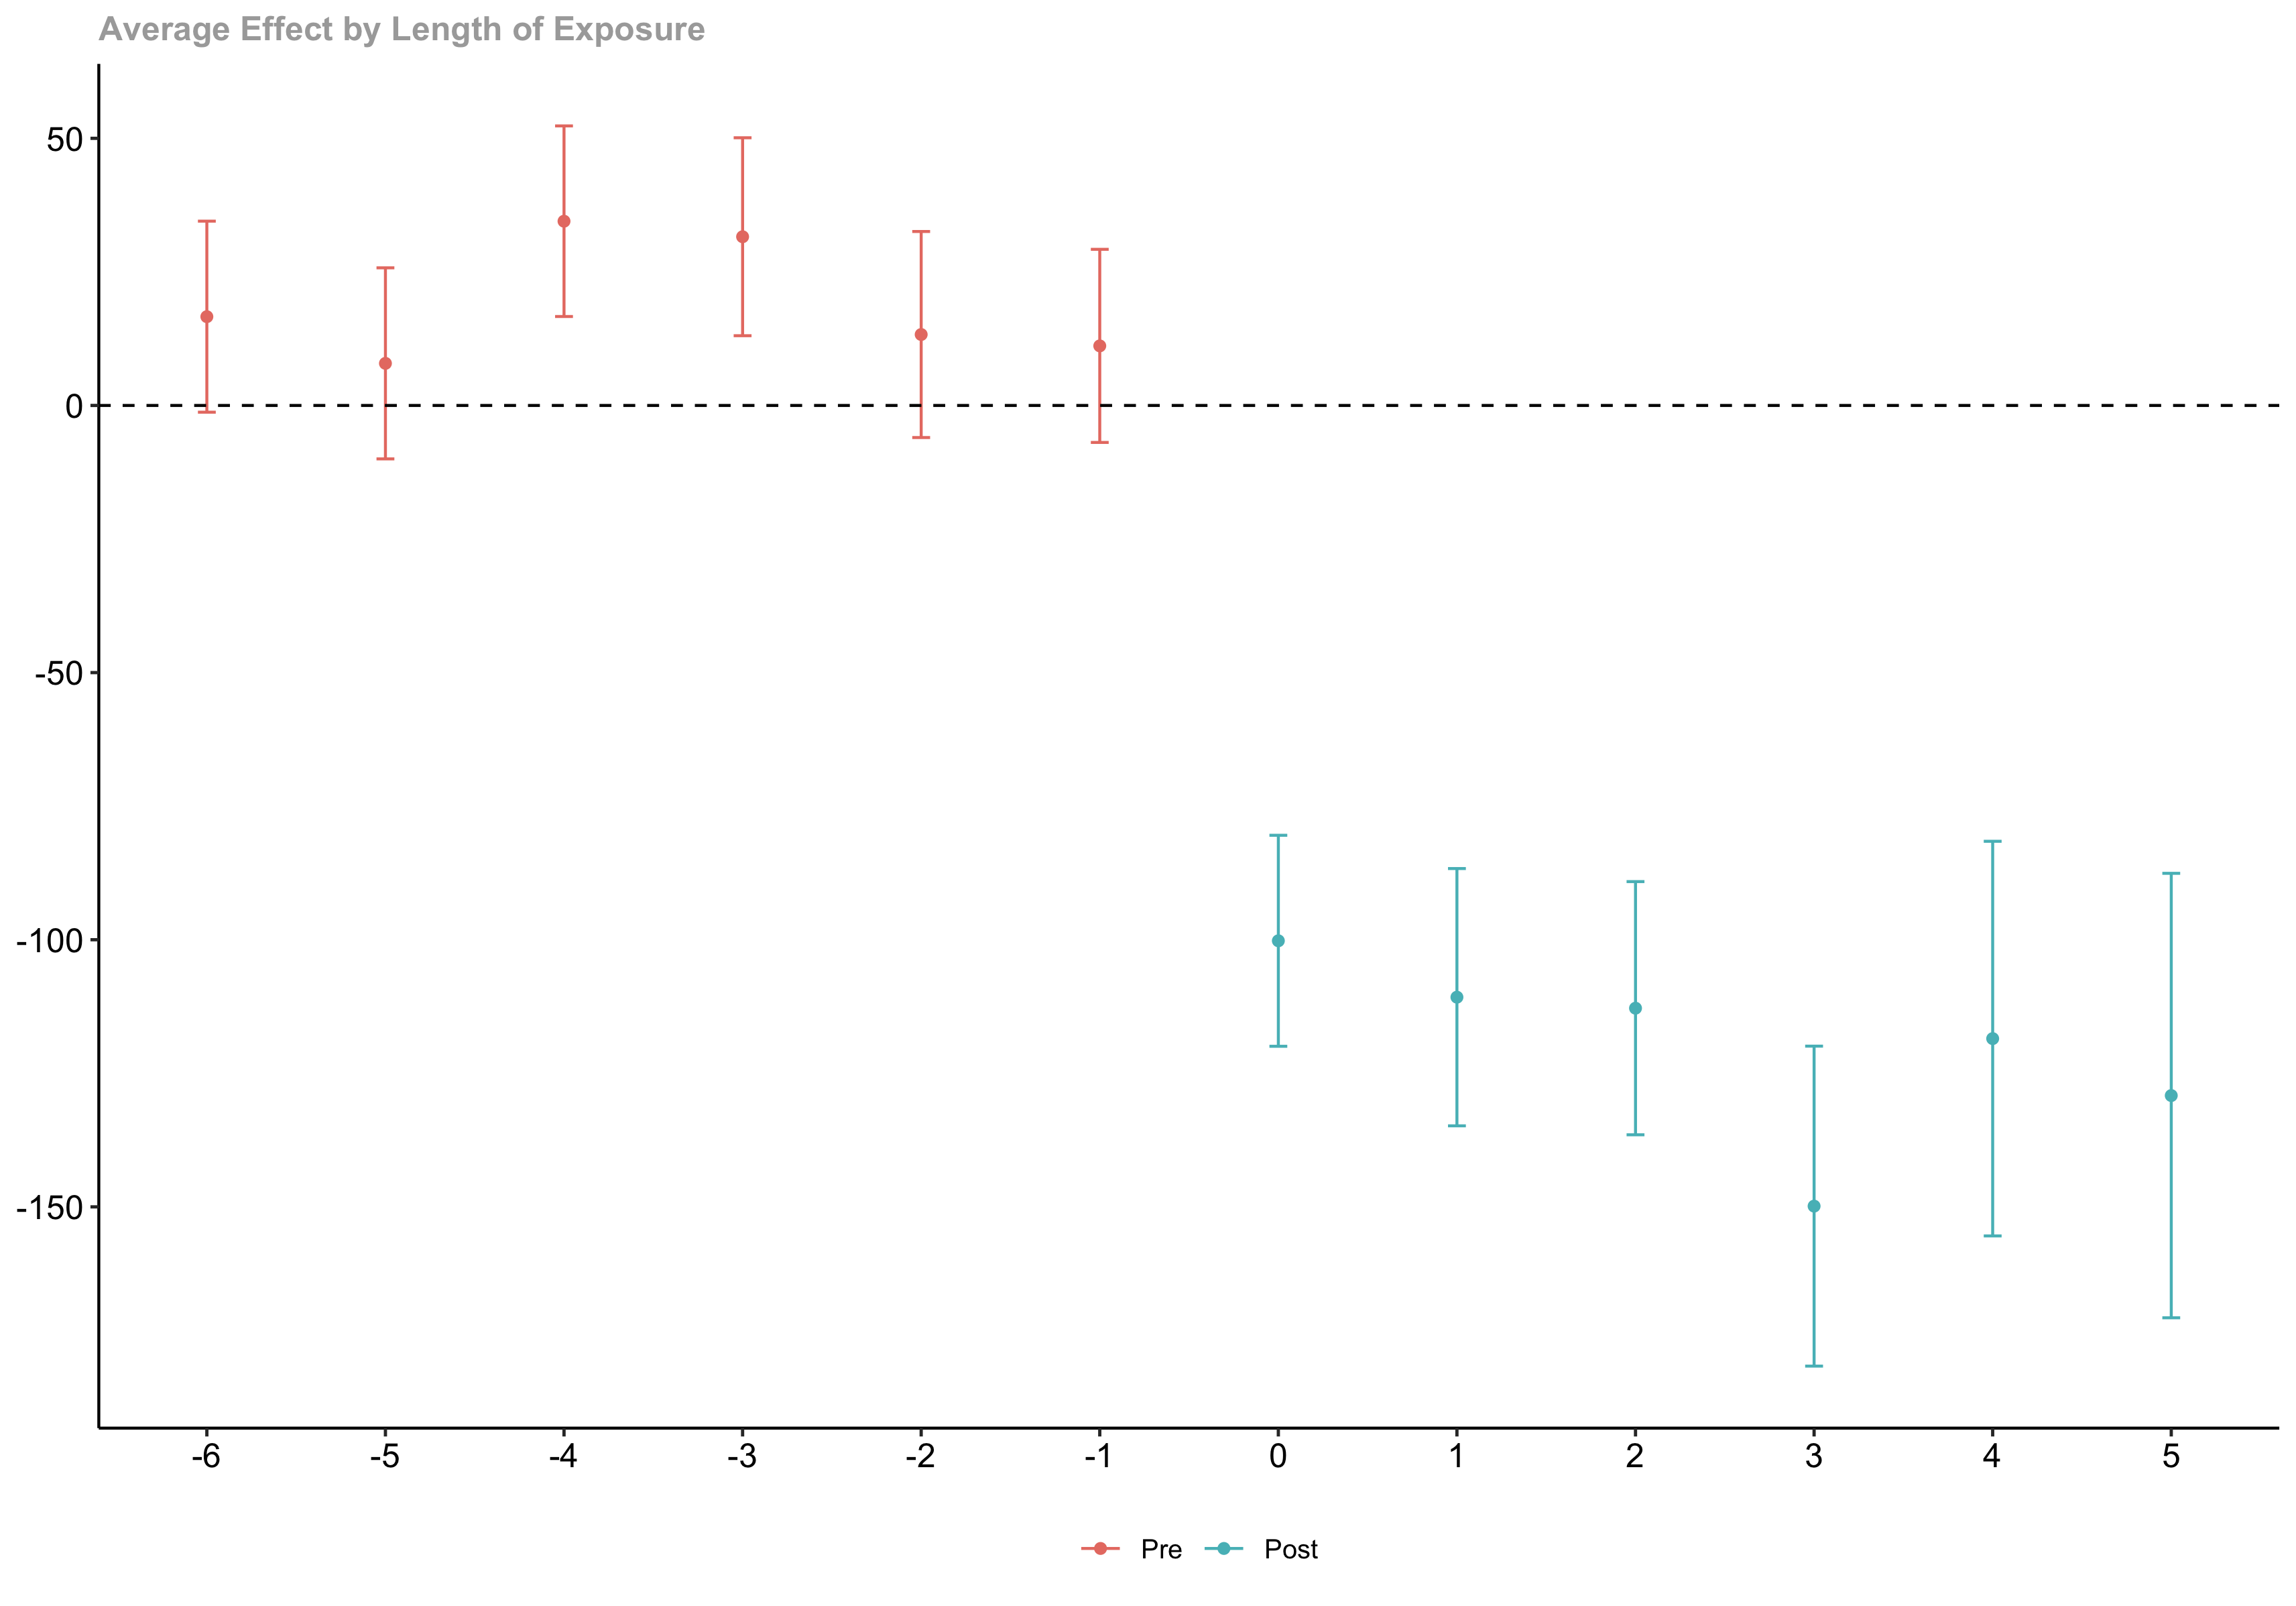
\includegraphics[width=.70\textwidth]{\figdir/bl_es.png}
    \fignote{\textwidth}{...}
\end{figure}


\subsection{Conditional parallel paths}%
\label{sub:conditional_parallel_paths}

Assumption:
\begin{itemize}
    \item Above, we assume that parallel paths hold for all units at all times.
    \item Here, we assume they hold for all units at all times with the same
        characteristics. (SA are the first to show that this works.)
\end{itemize}

Notes:
\begin{itemize}
    \item We wouldn't expect conditional parallel trends. If we think that
        discretionary spend is constant fraction of income or total spend, then
        this implies parallel trends in the variables we control for.

    \item Same with number of accounts: average spend from account is constant,
        then dspend has parallel trends in the number of accounts.
\end{itemize}

\begin{figure}[H]
    \centering
    \caption{New results}%
    \label{fig:new}
    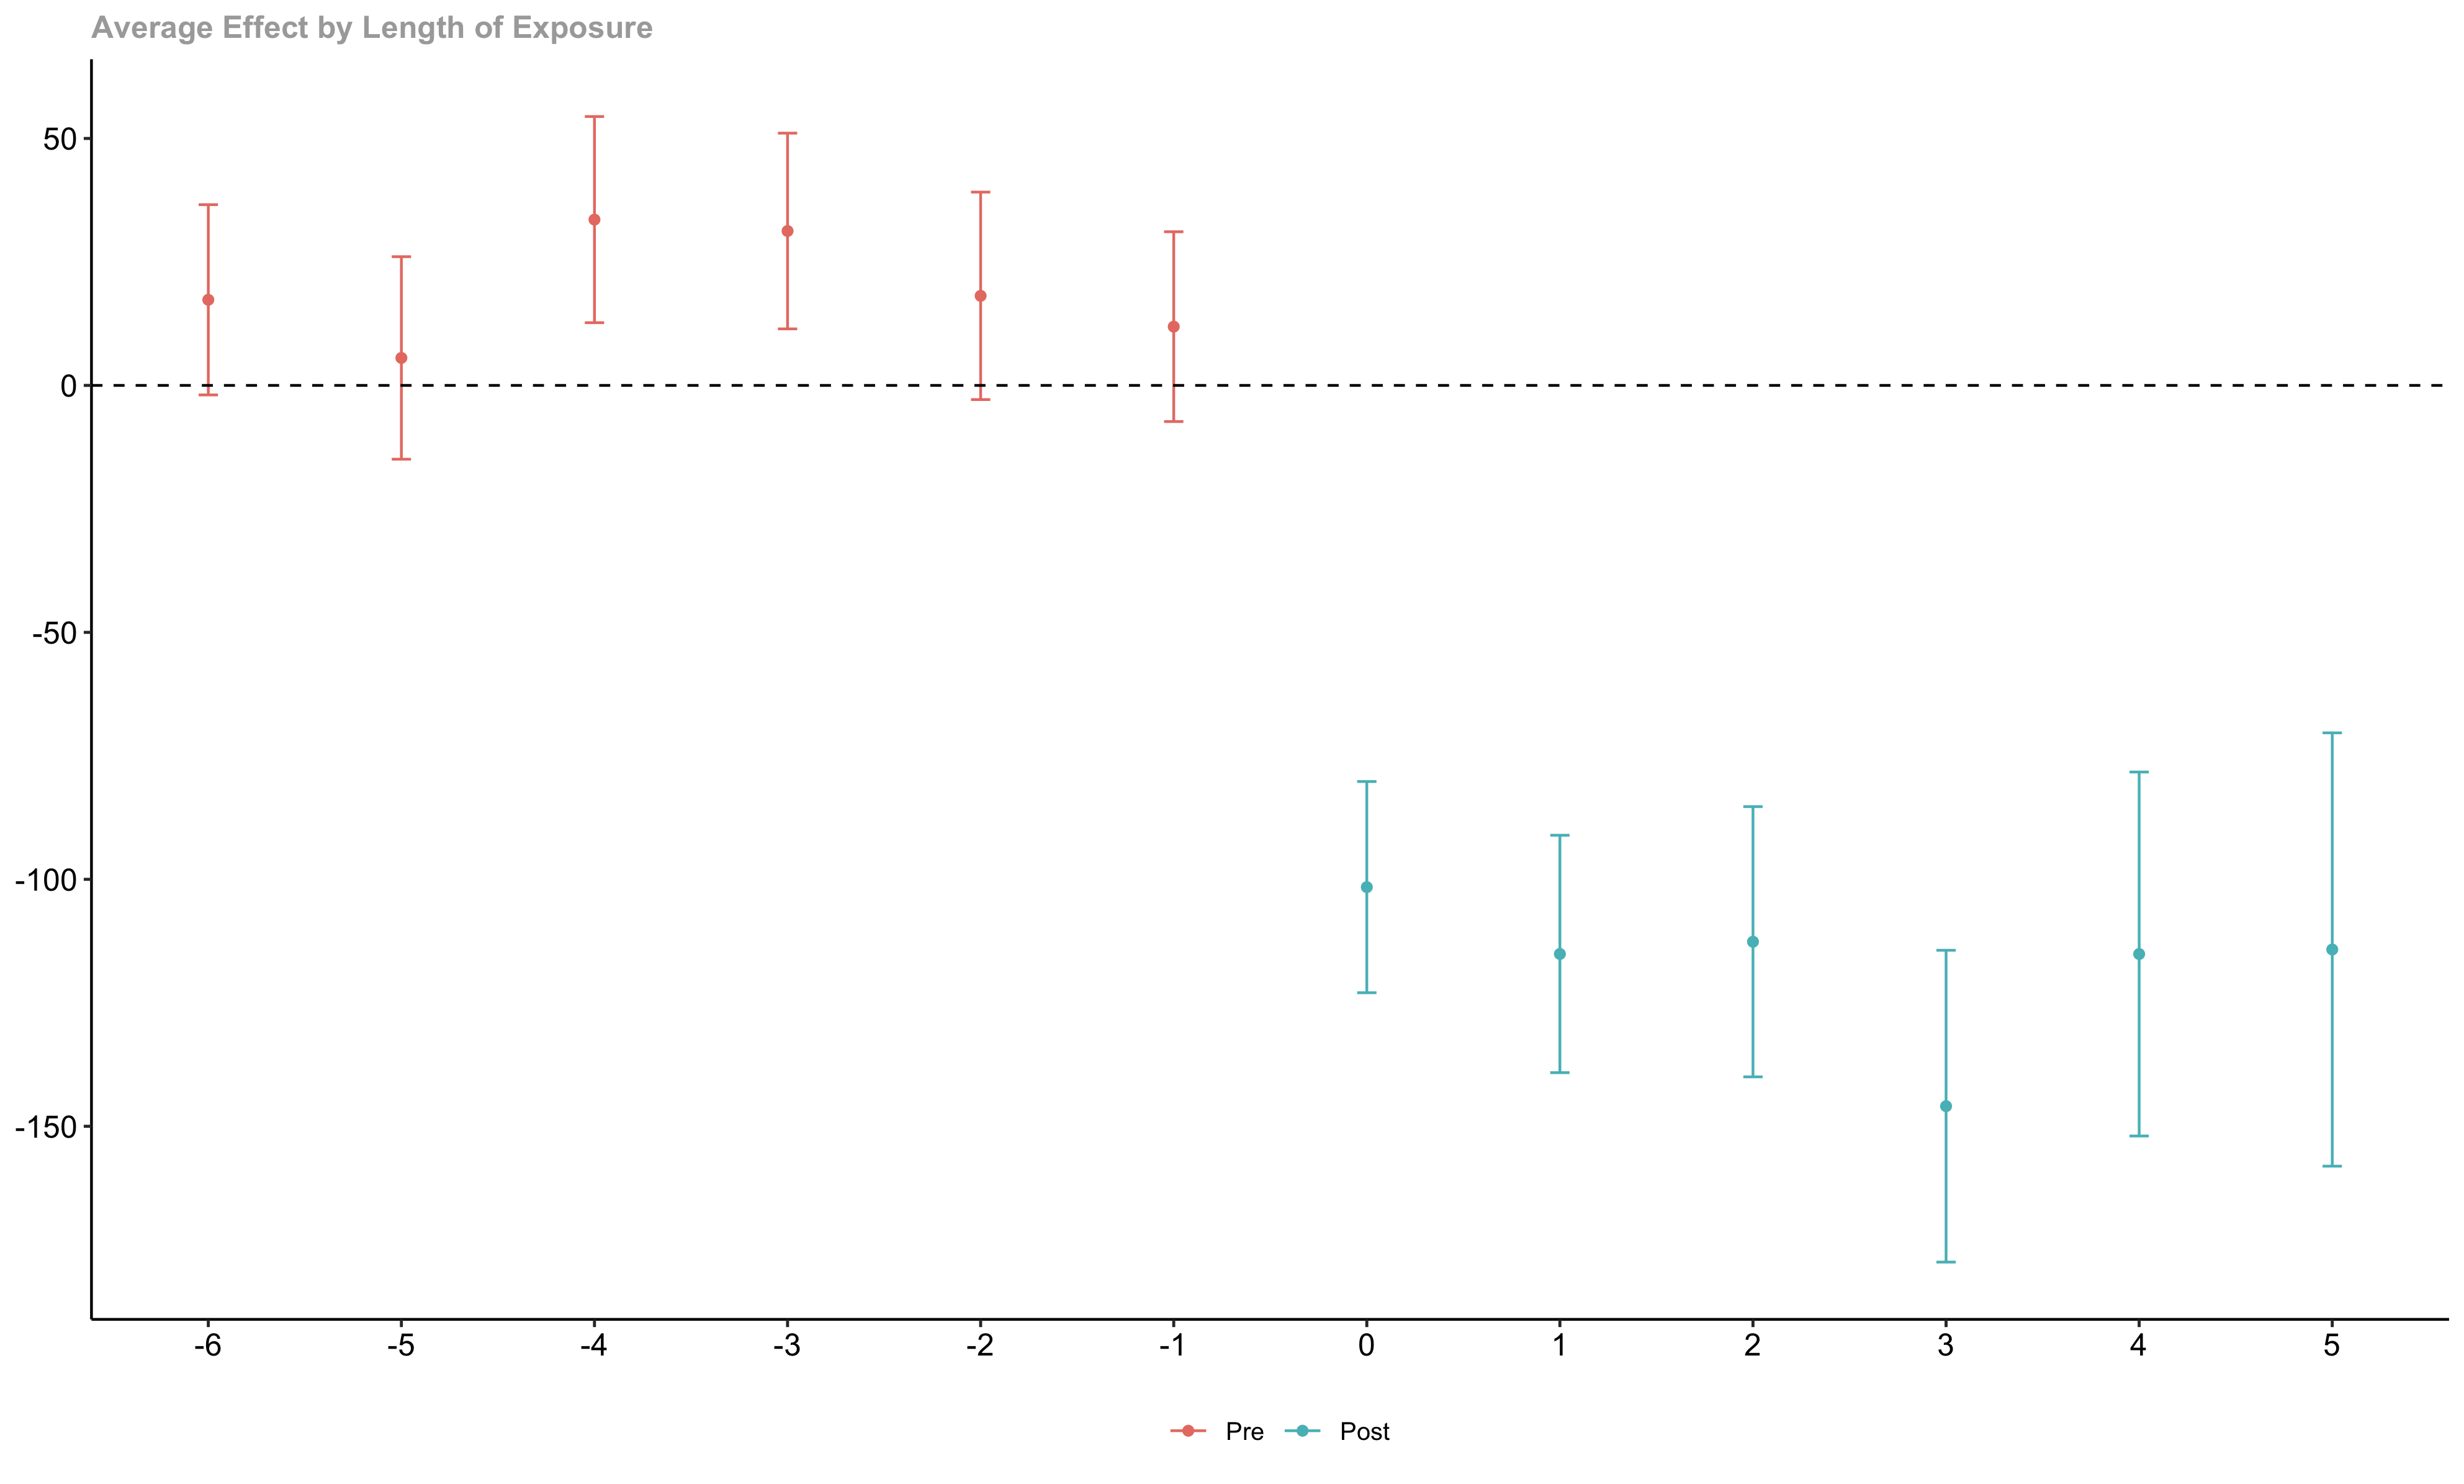
\includegraphics[width=.70\textwidth]{\figdir/cond_es.png}
    \fignote{\textwidth}{...}
\end{figure}


\subsection{Relaxing anticipation assumption}%
\label{sub:relaxing_anticipation_assumption}

See callaway2021difference-appendix for discussion.

\begin{figure}[H]
    \centering
    \caption{New results}%
    \label{fig:new}
    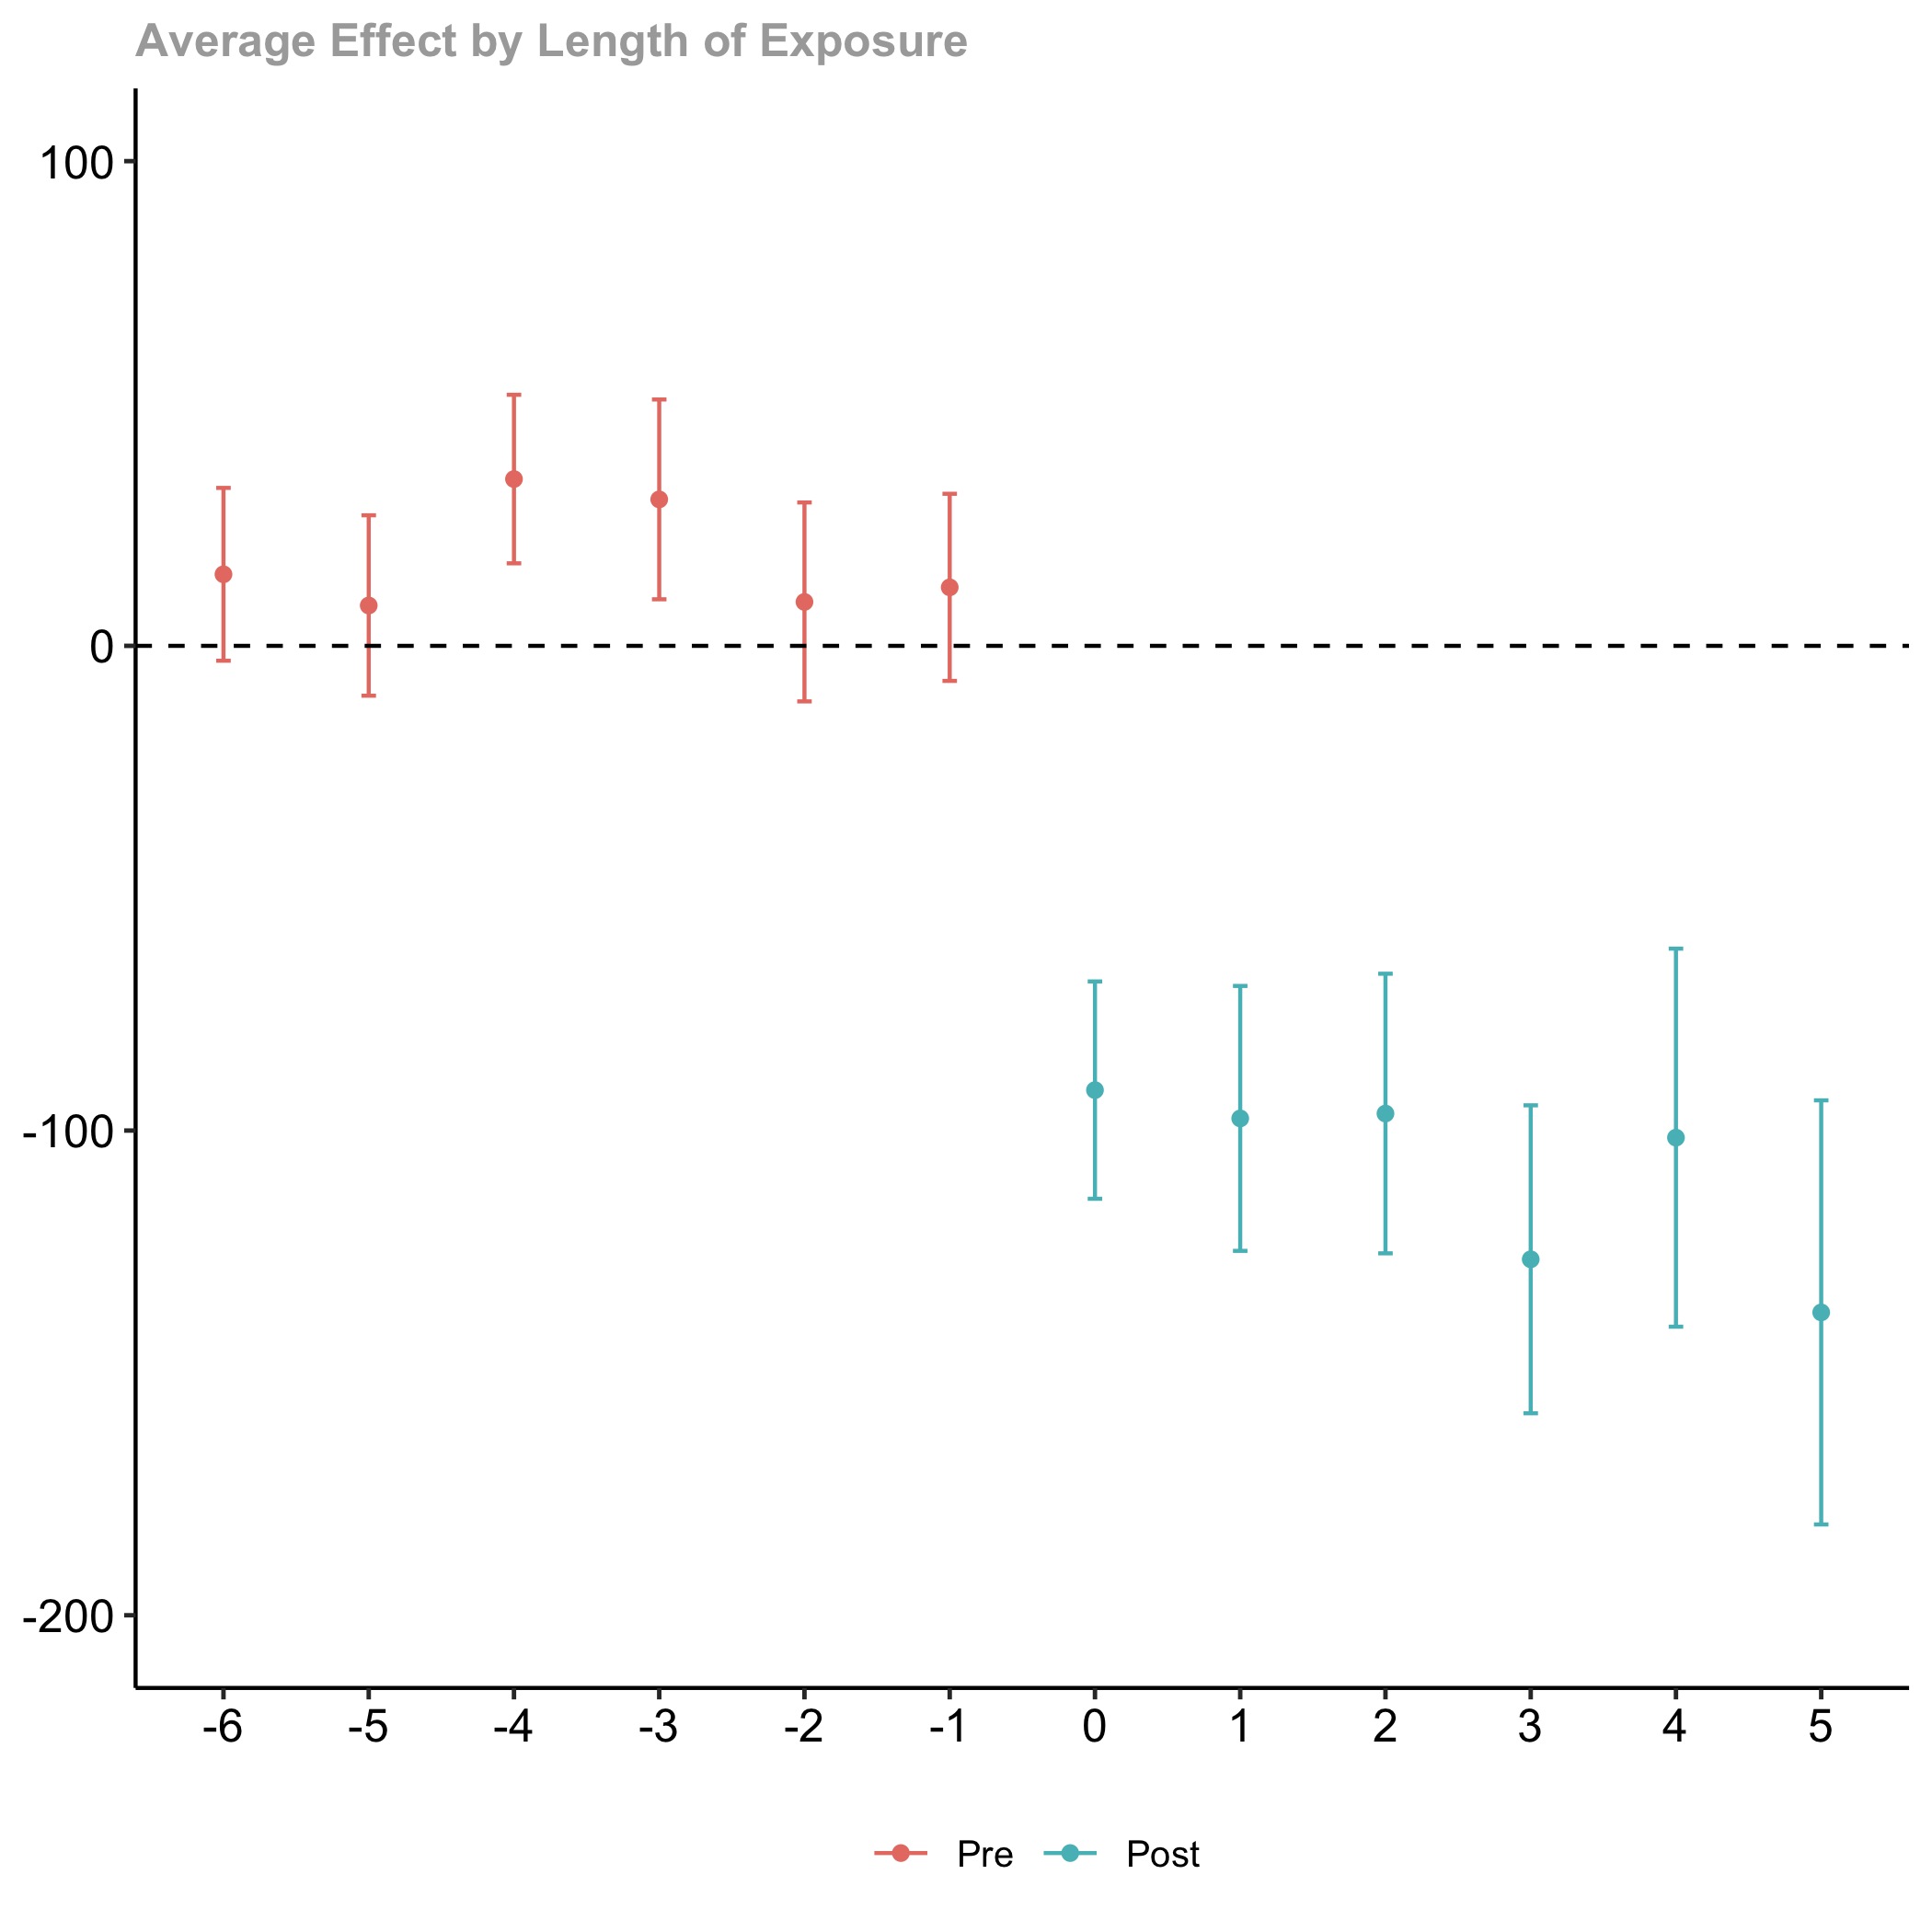
\includegraphics[width=.32\textwidth]{\figdir/antic1_es.png}
    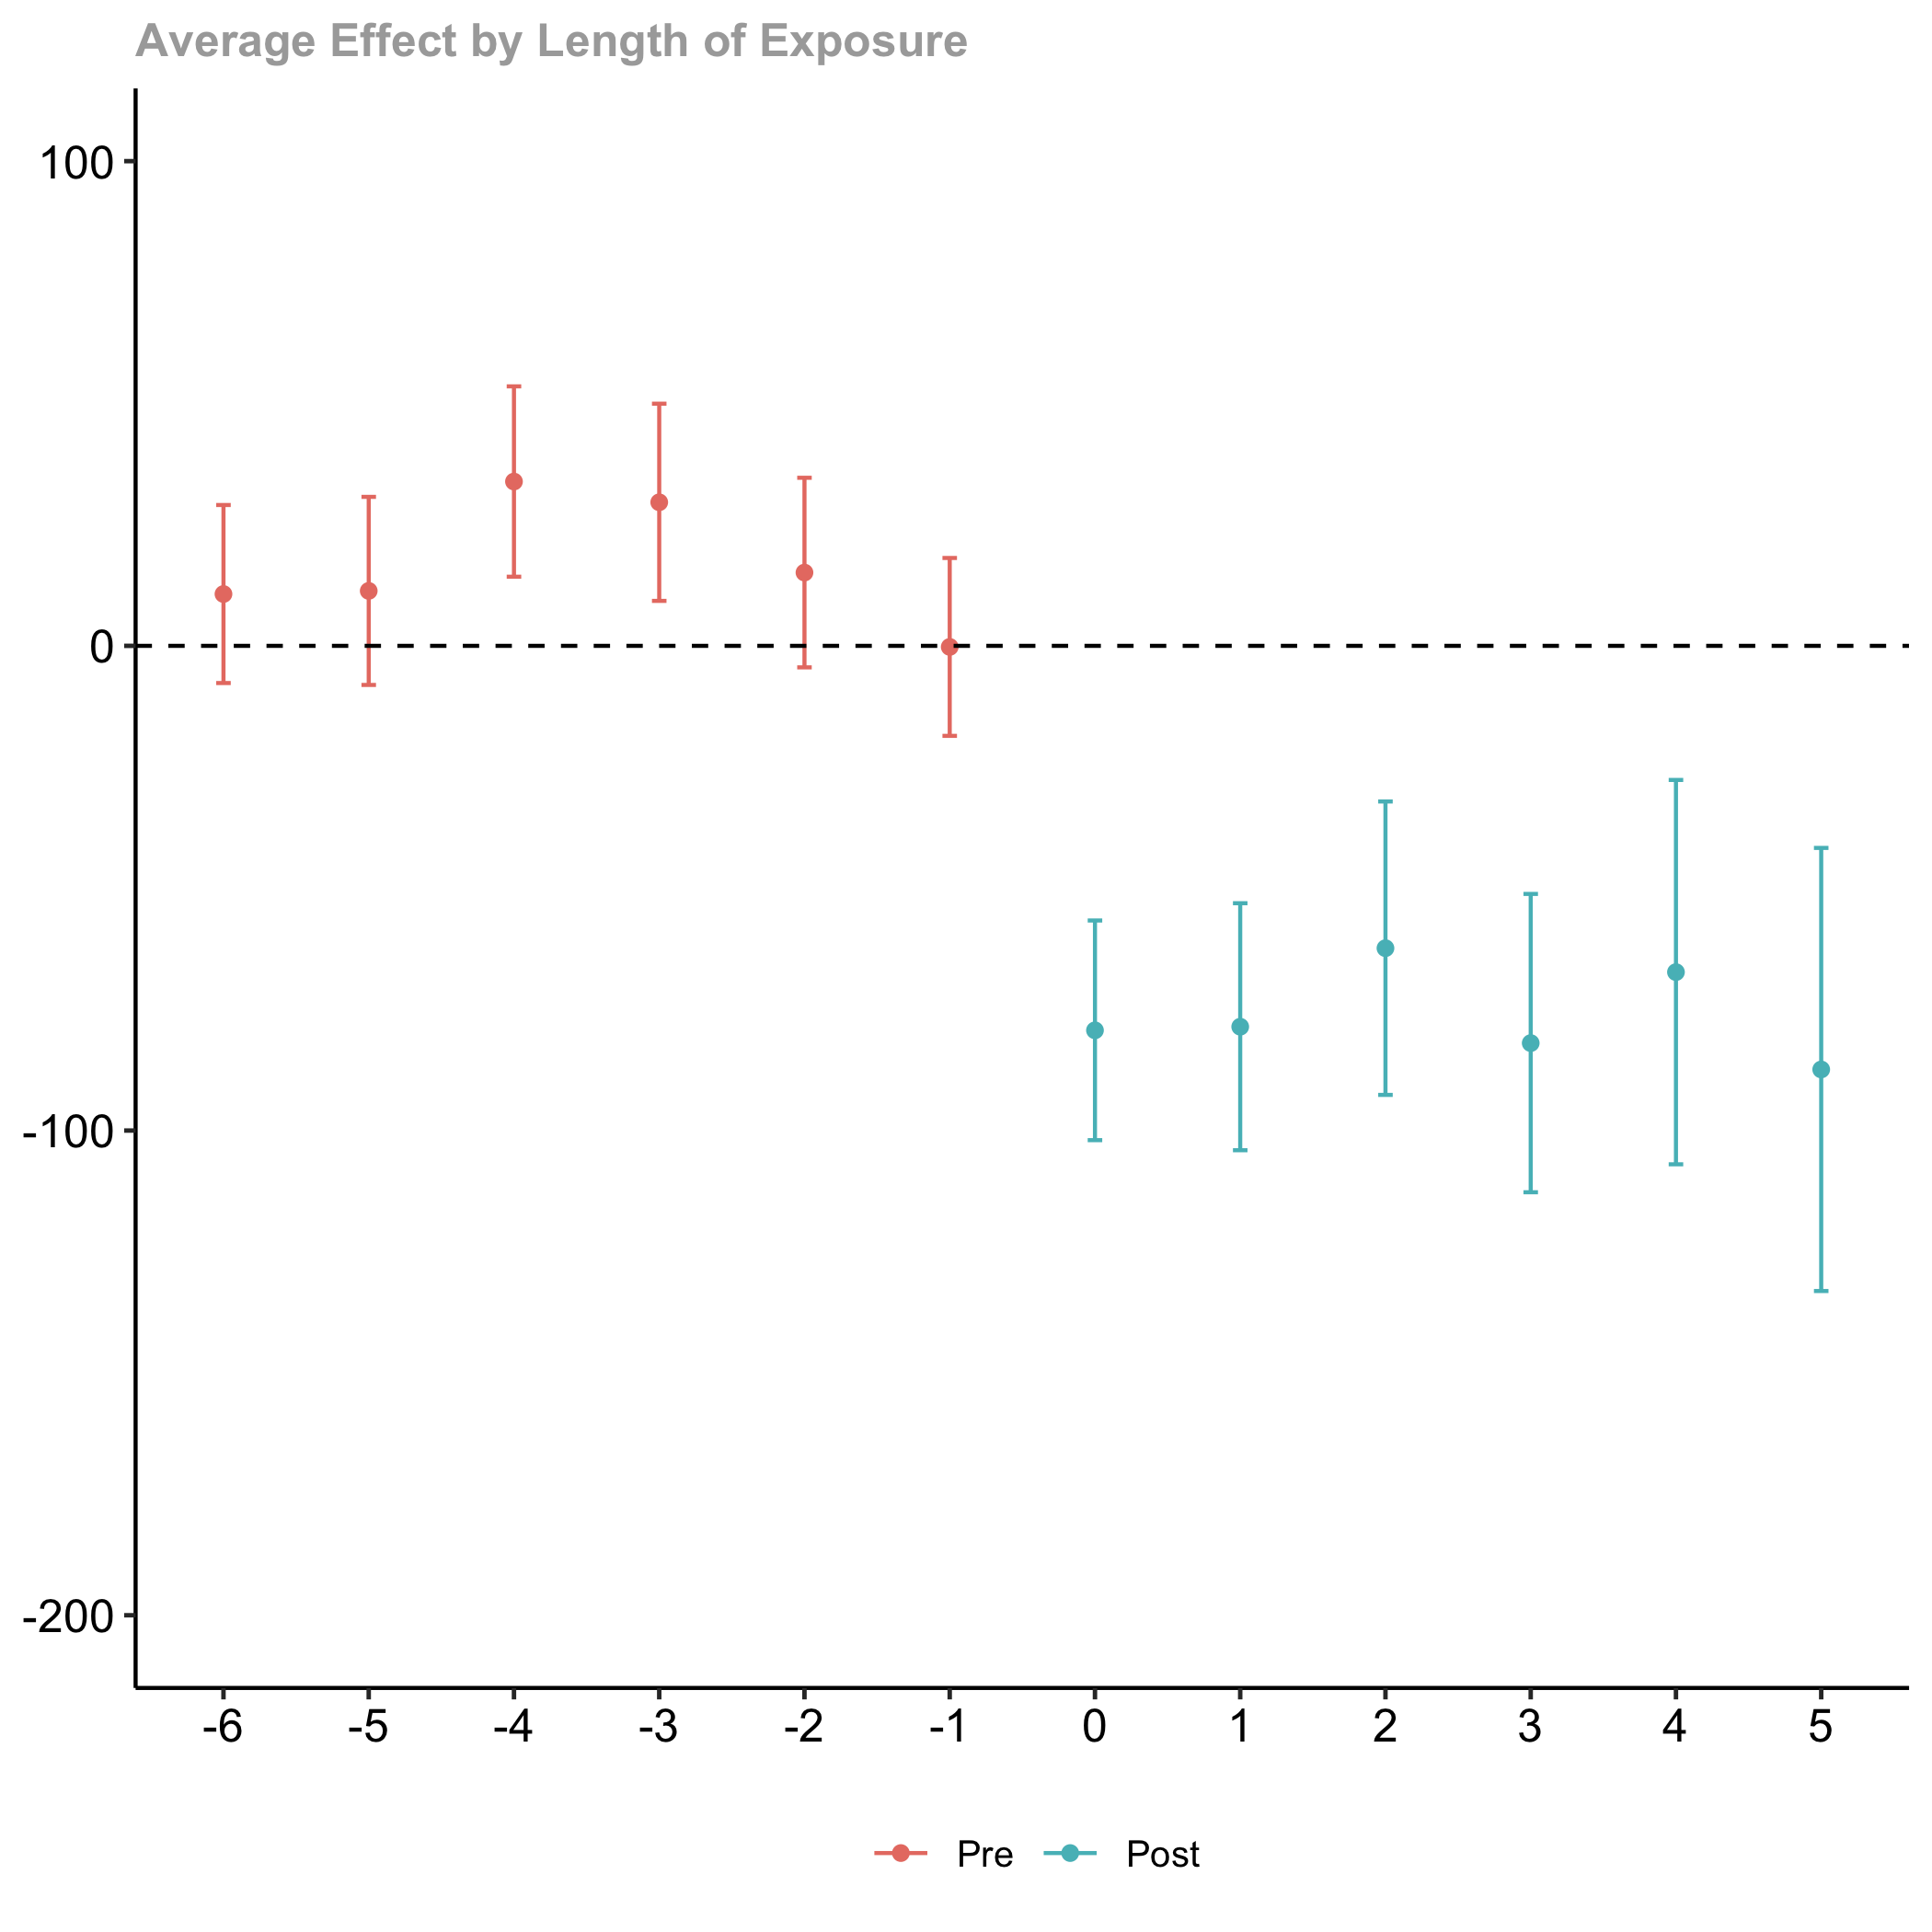
\includegraphics[width=.32\textwidth]{\figdir/antic2_es.png}
    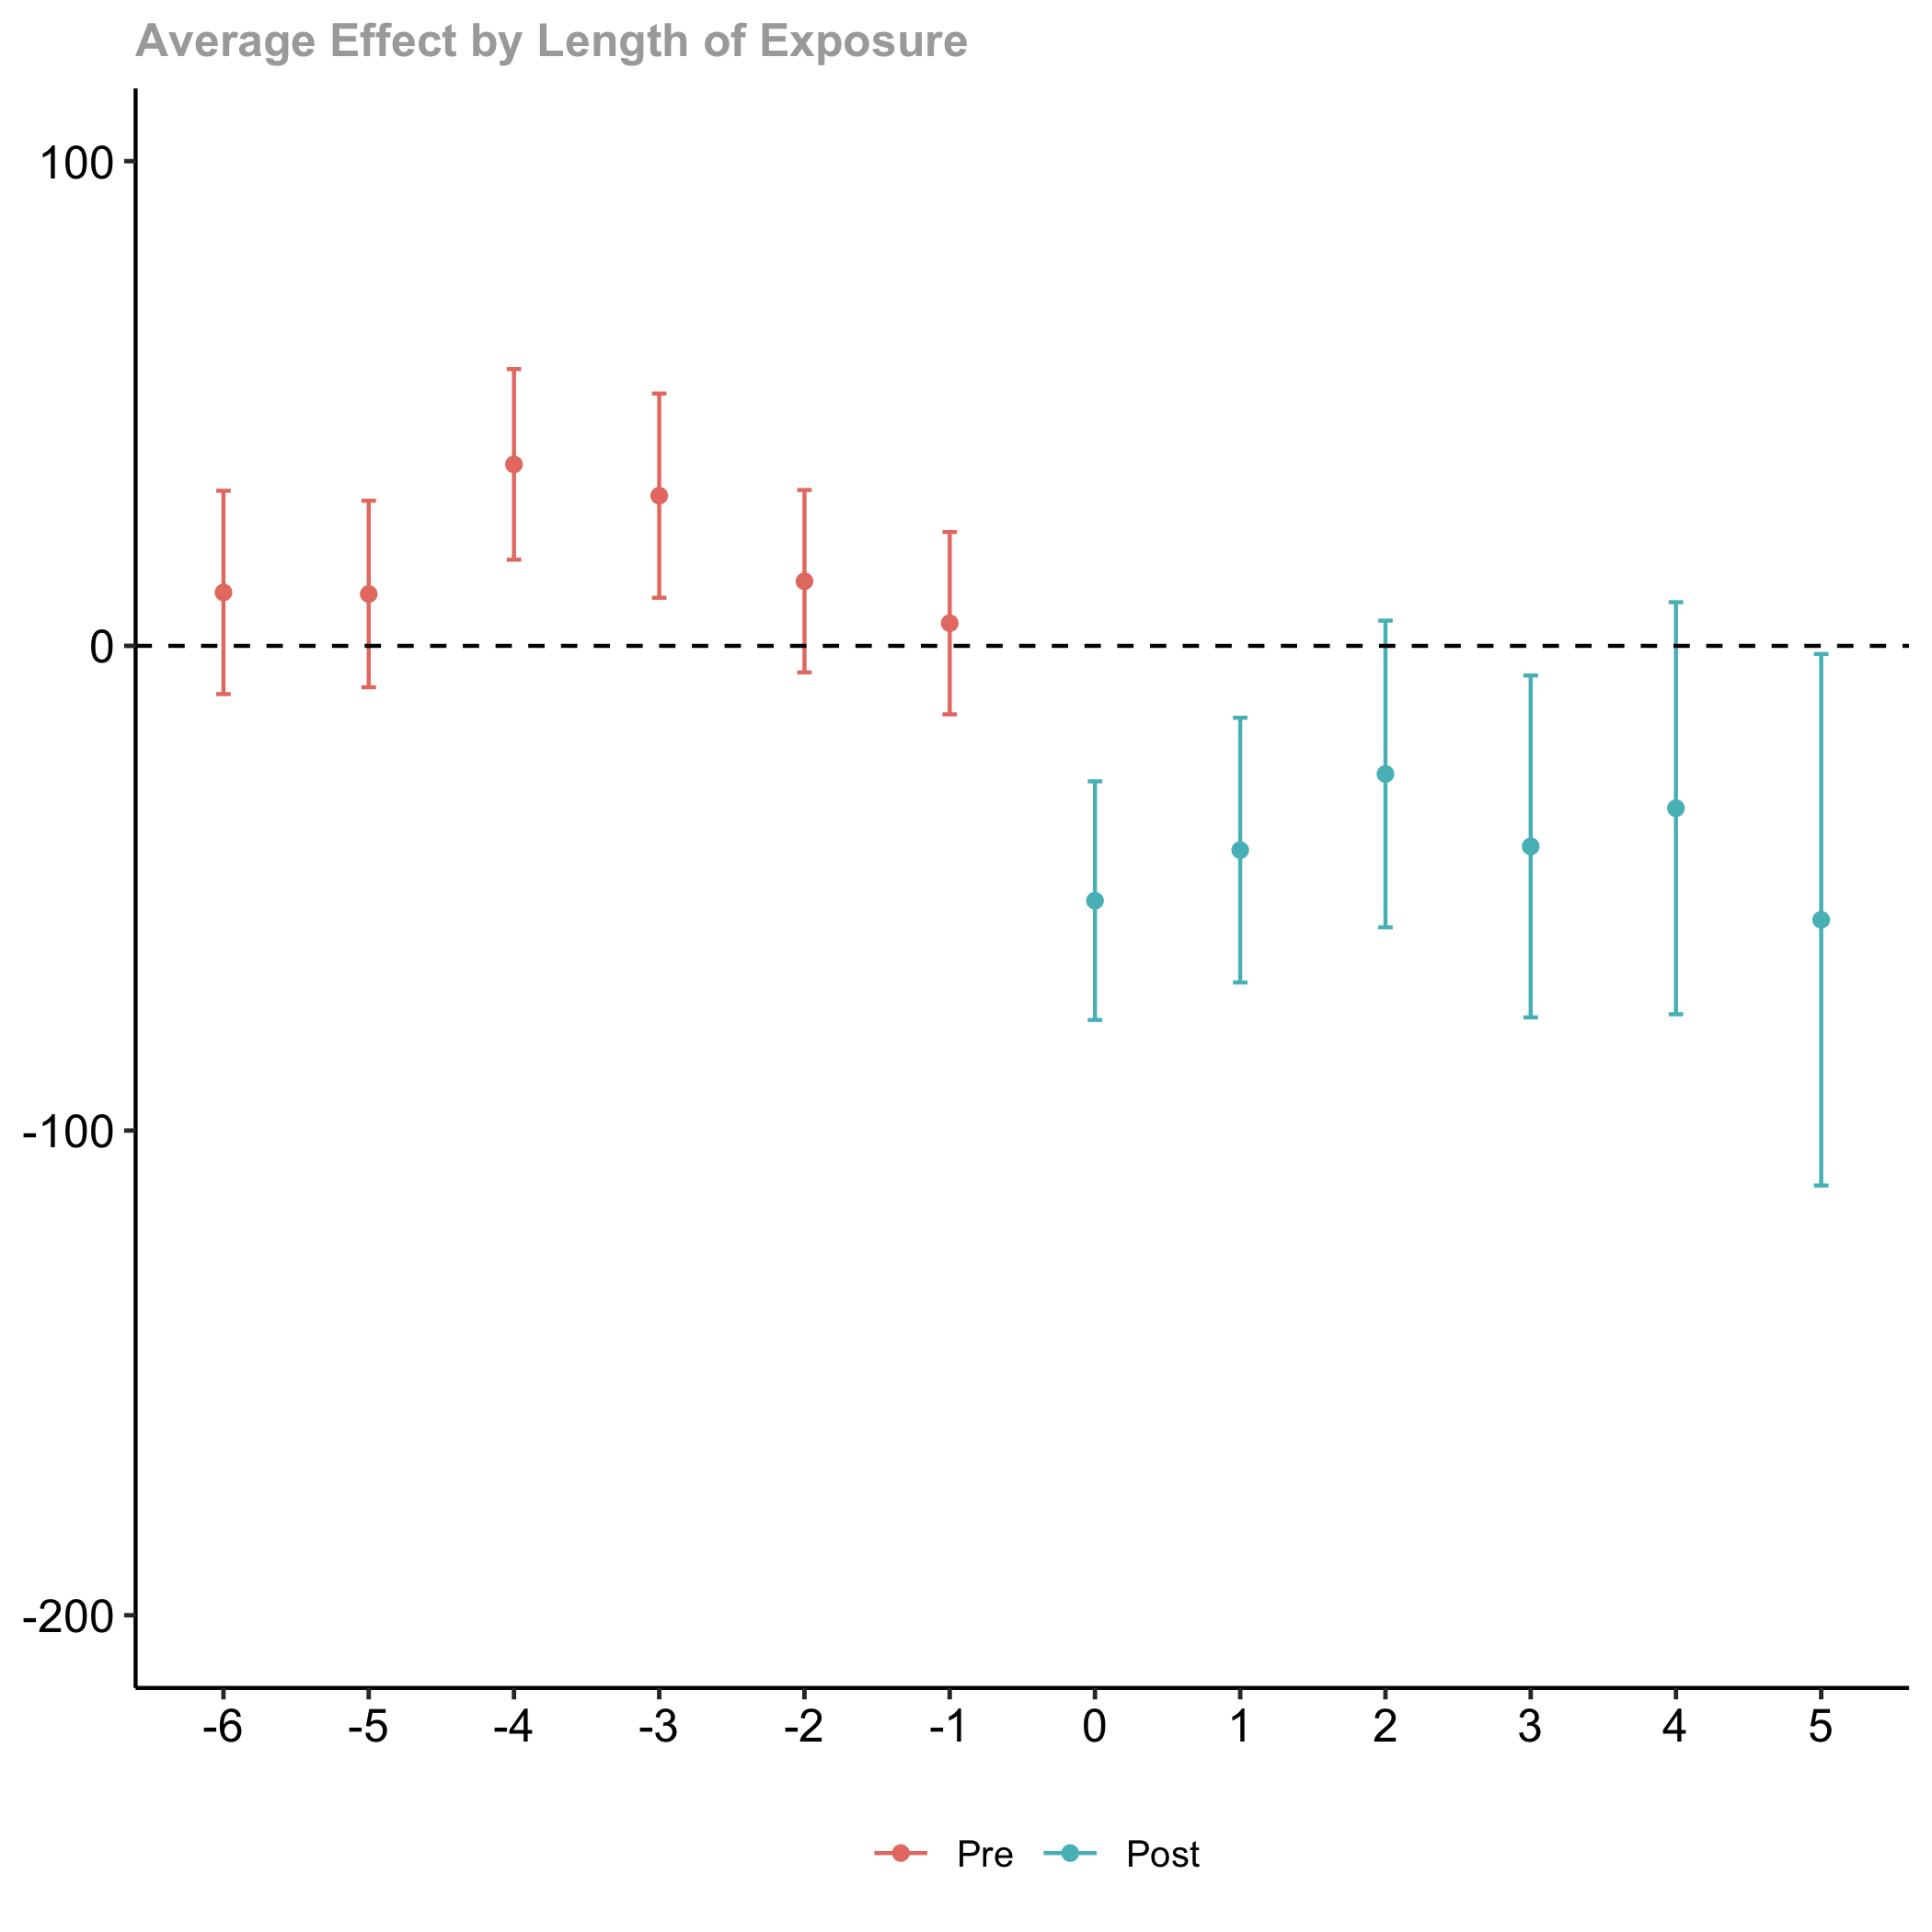
\includegraphics[width=.32\textwidth]{\figdir/antic3_es.png}
    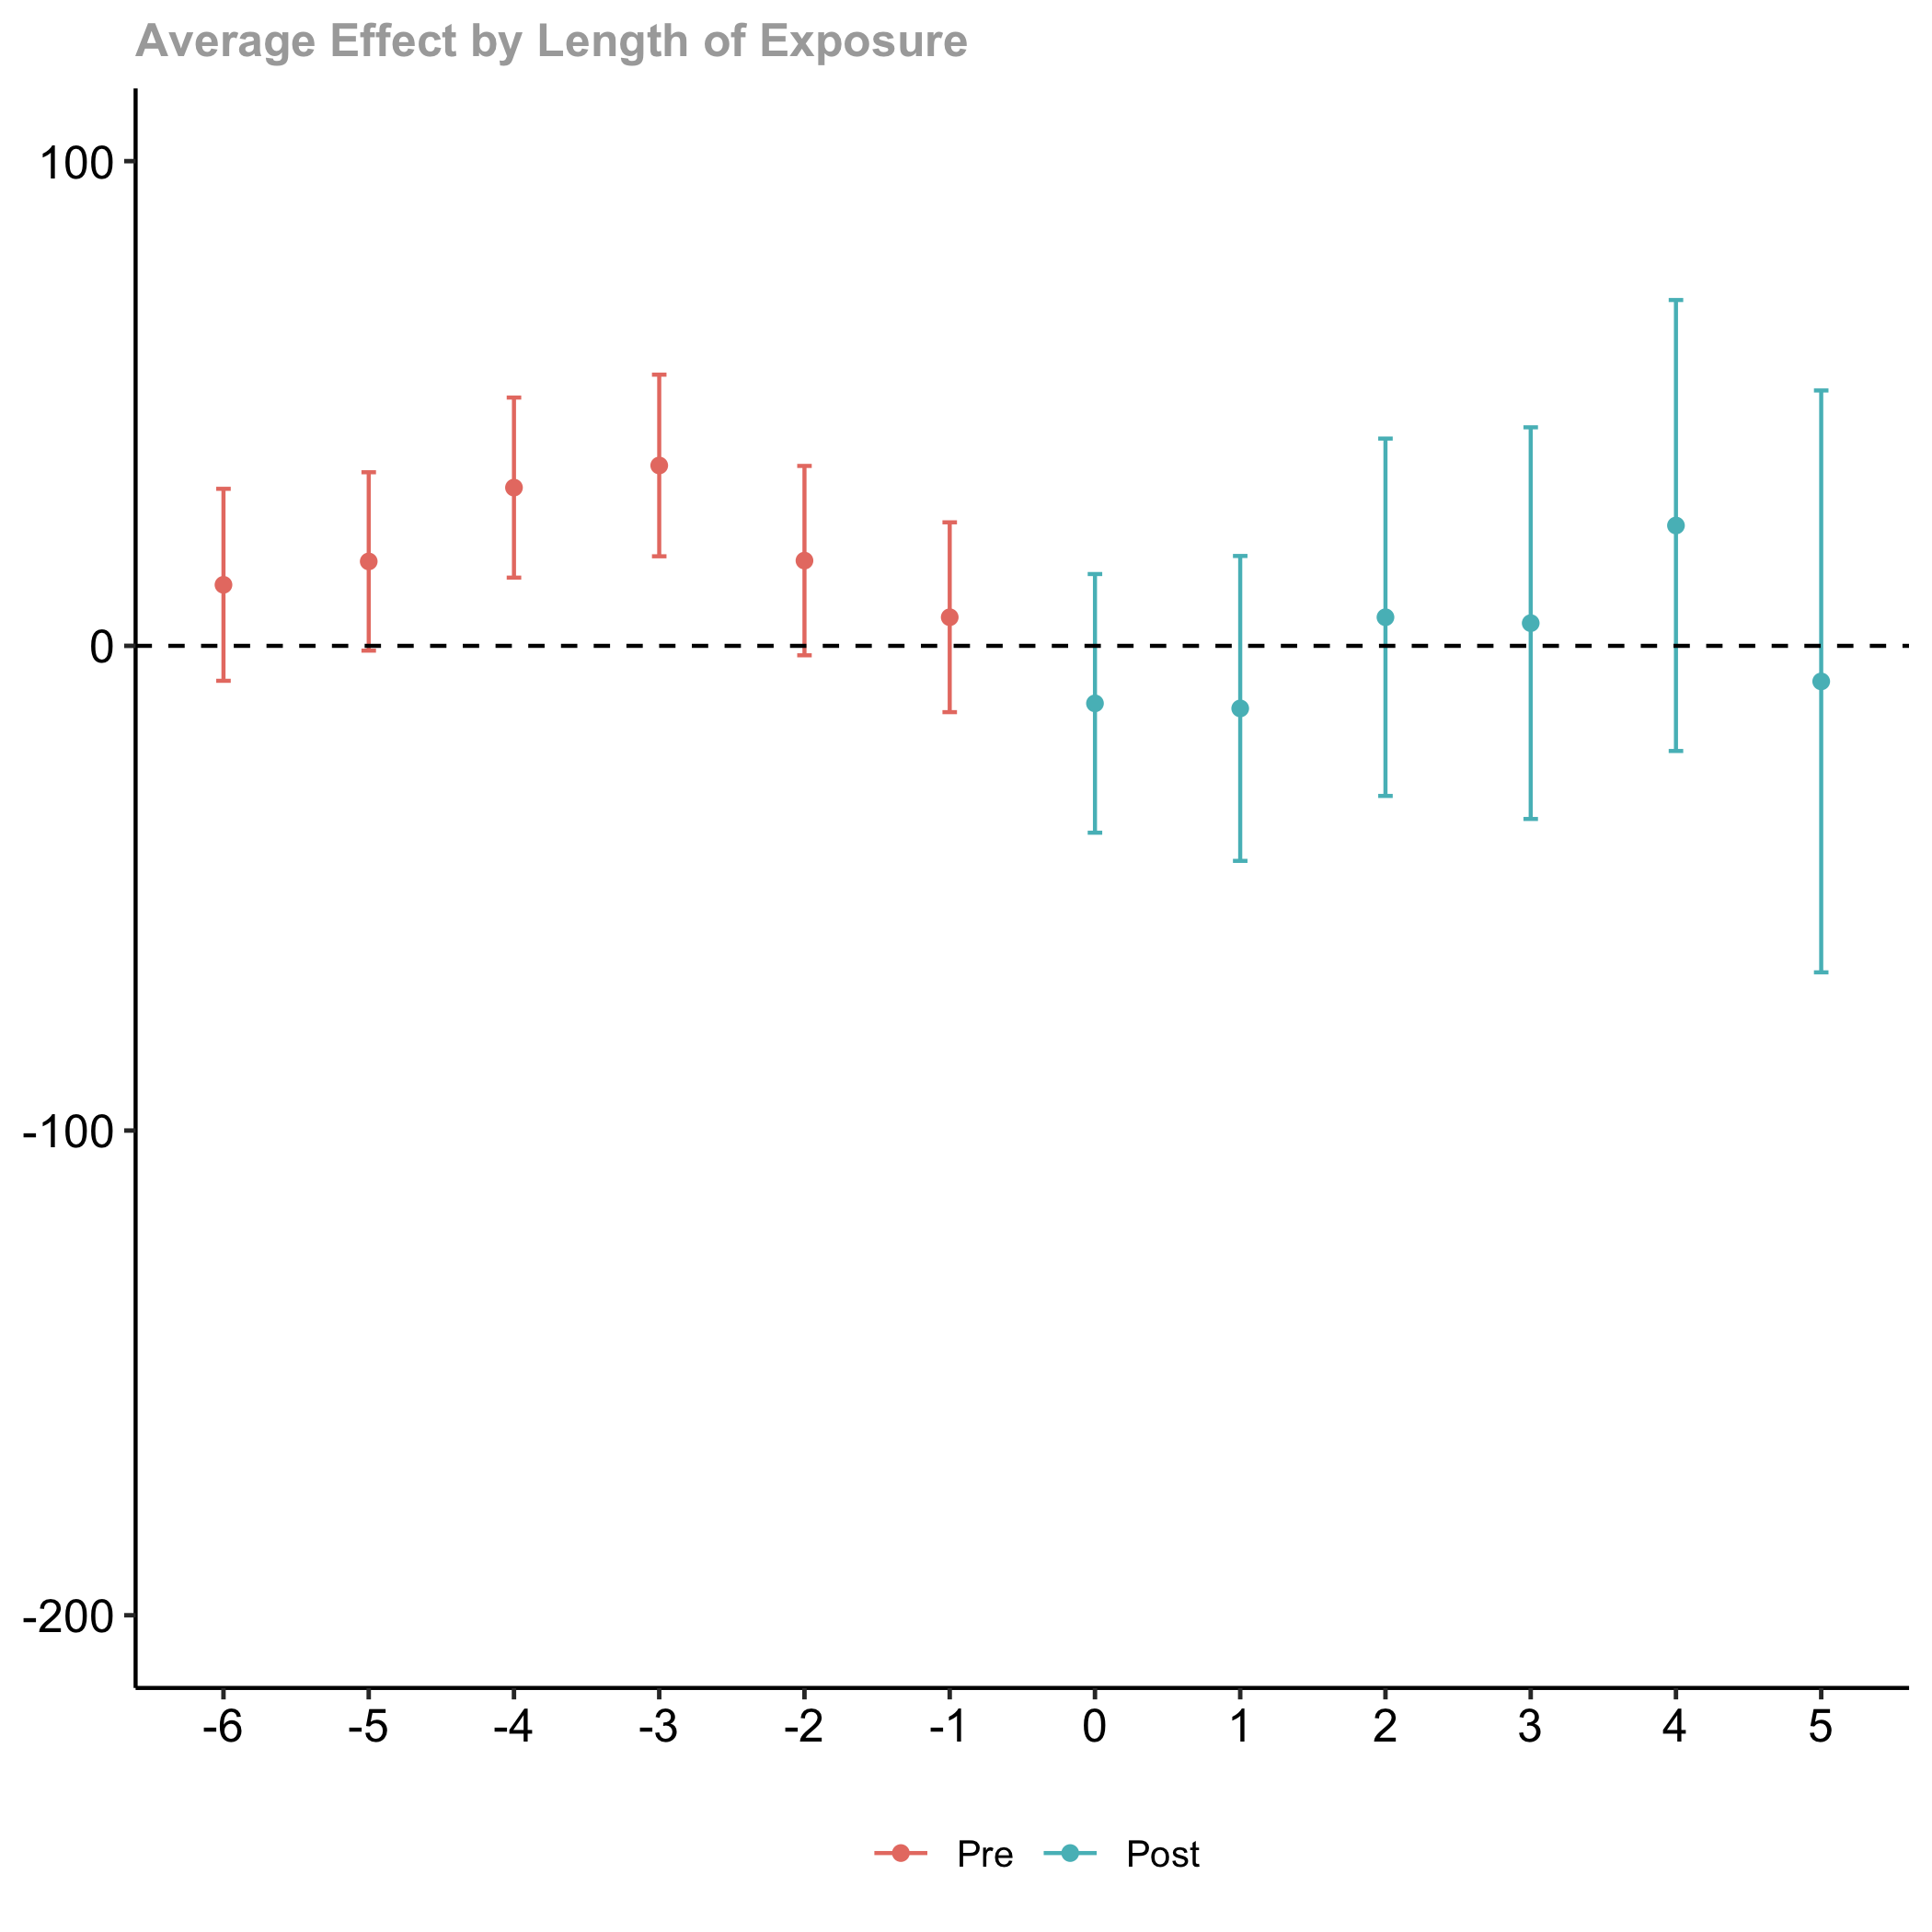
\includegraphics[width=.32\textwidth]{\figdir/antic4_es.png}
    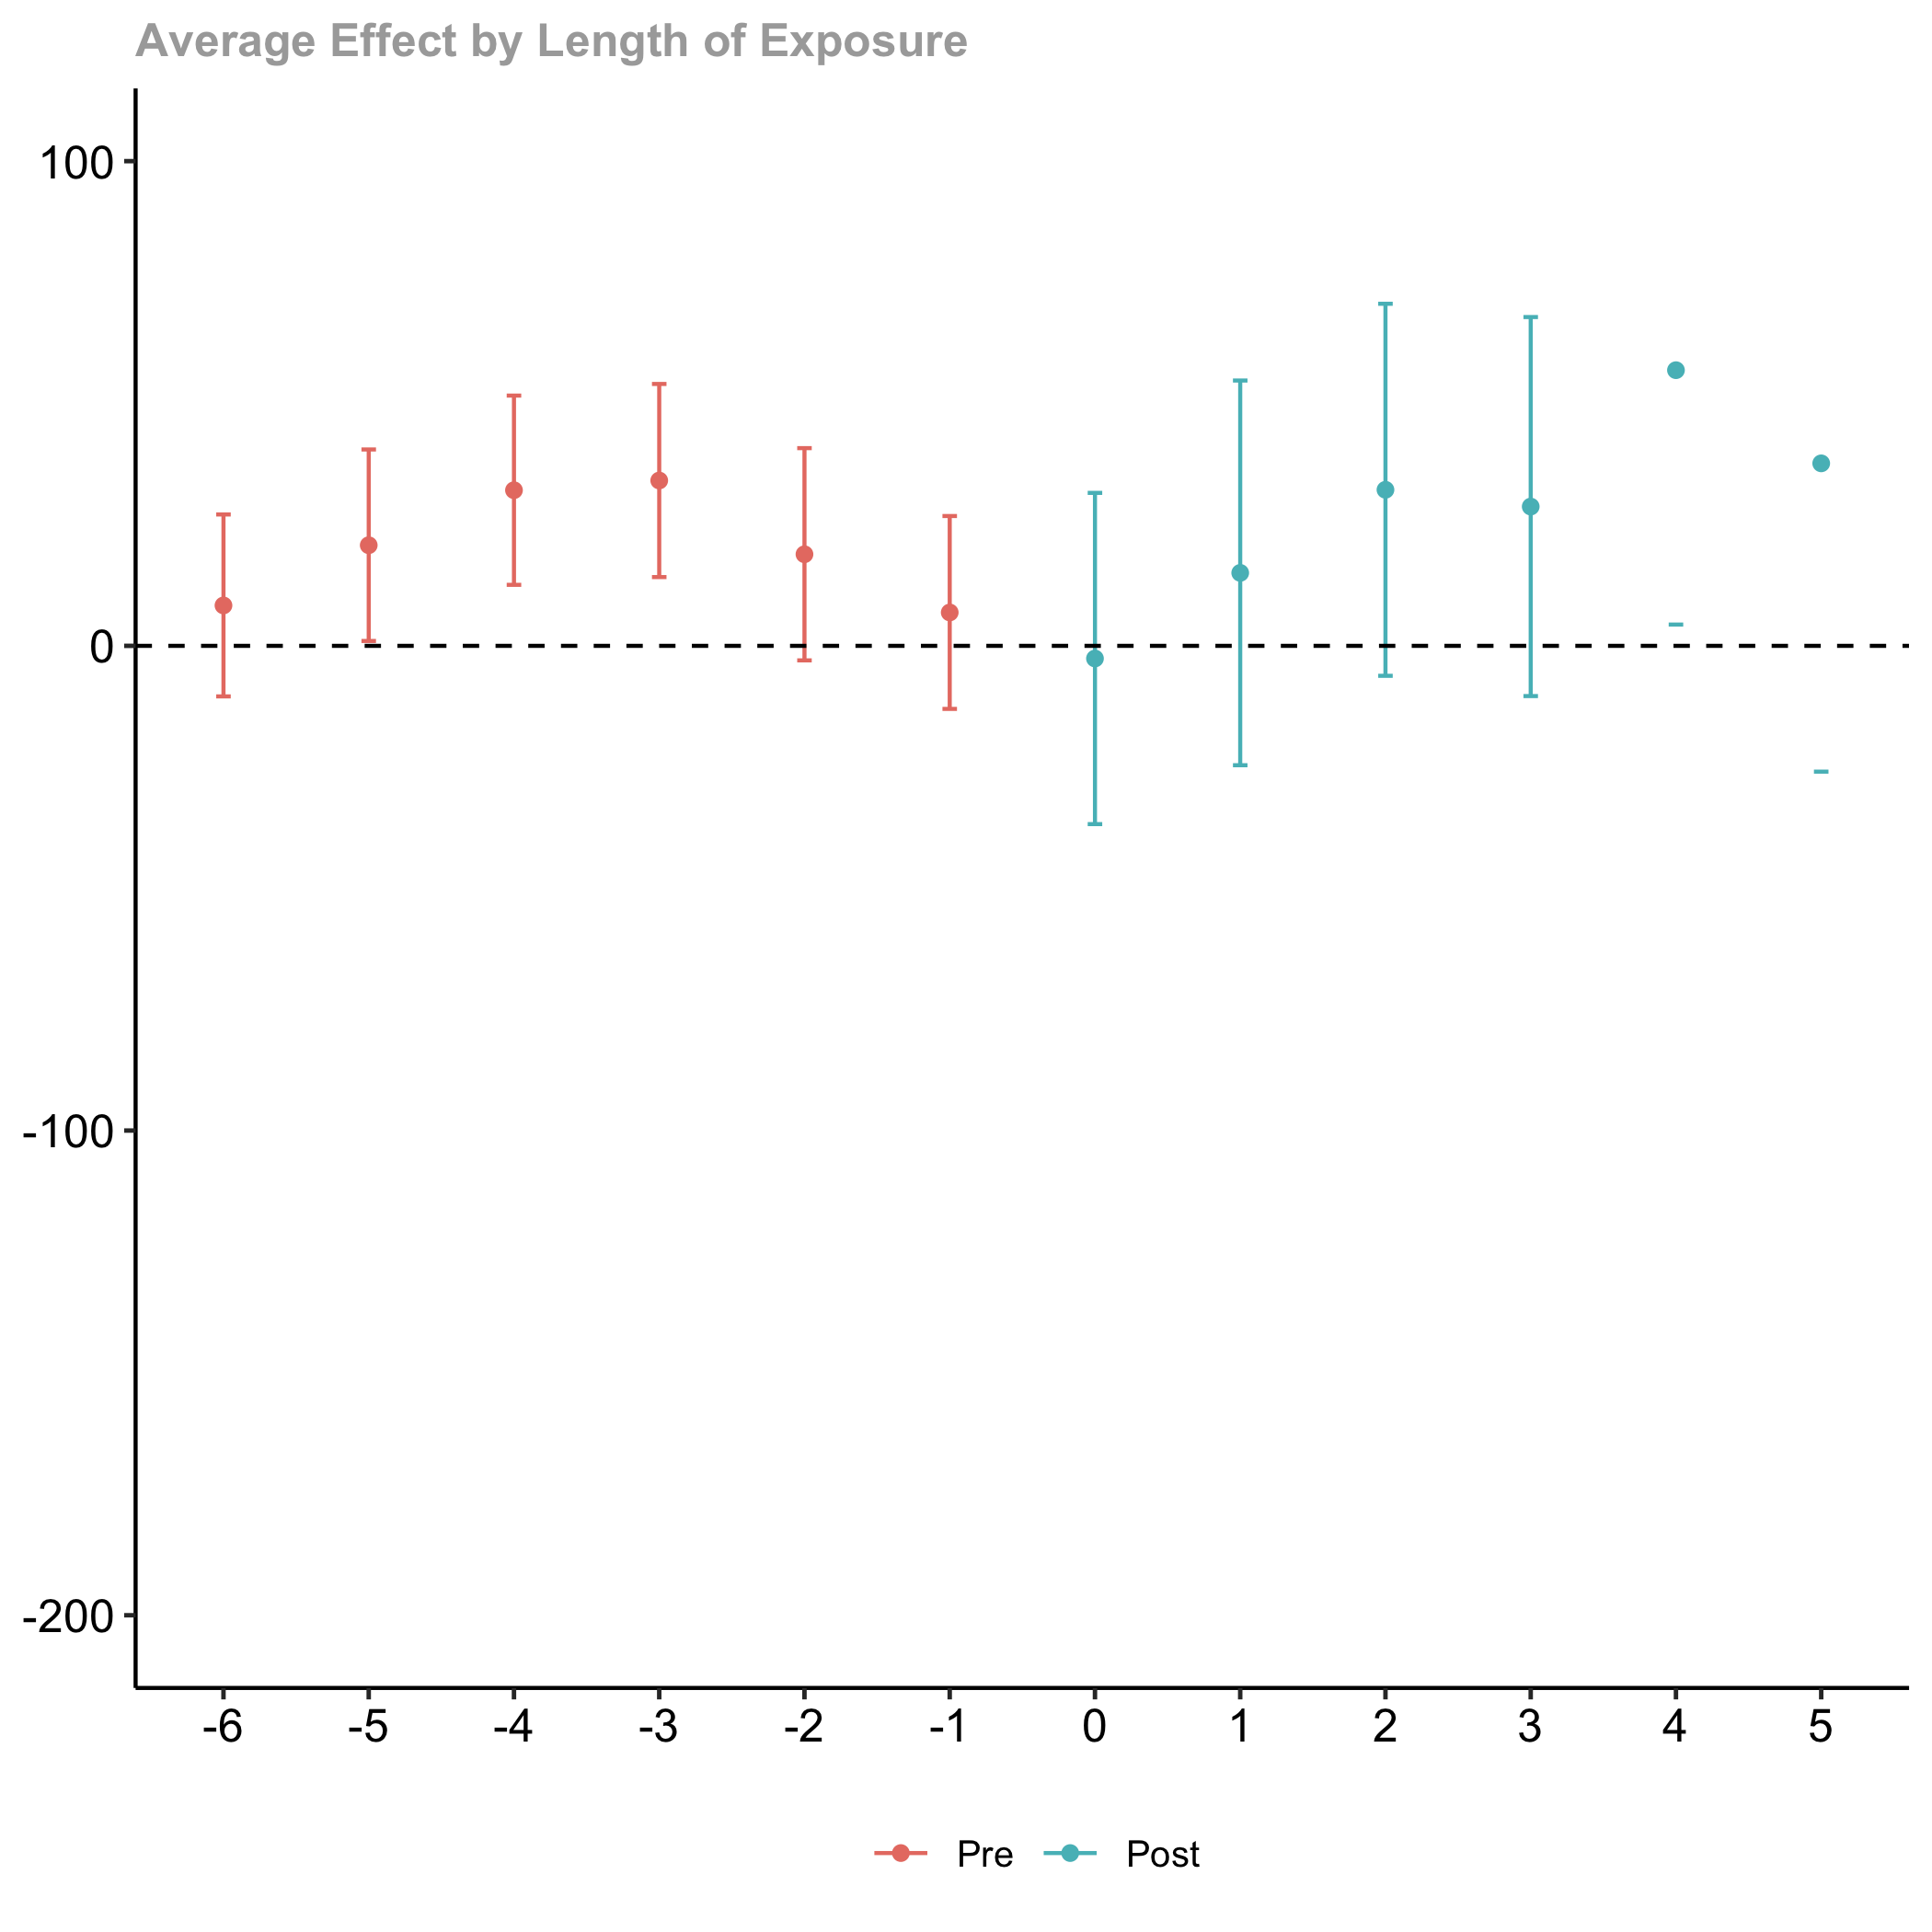
\includegraphics[width=.32\textwidth]{\figdir/antic5_es.png}
    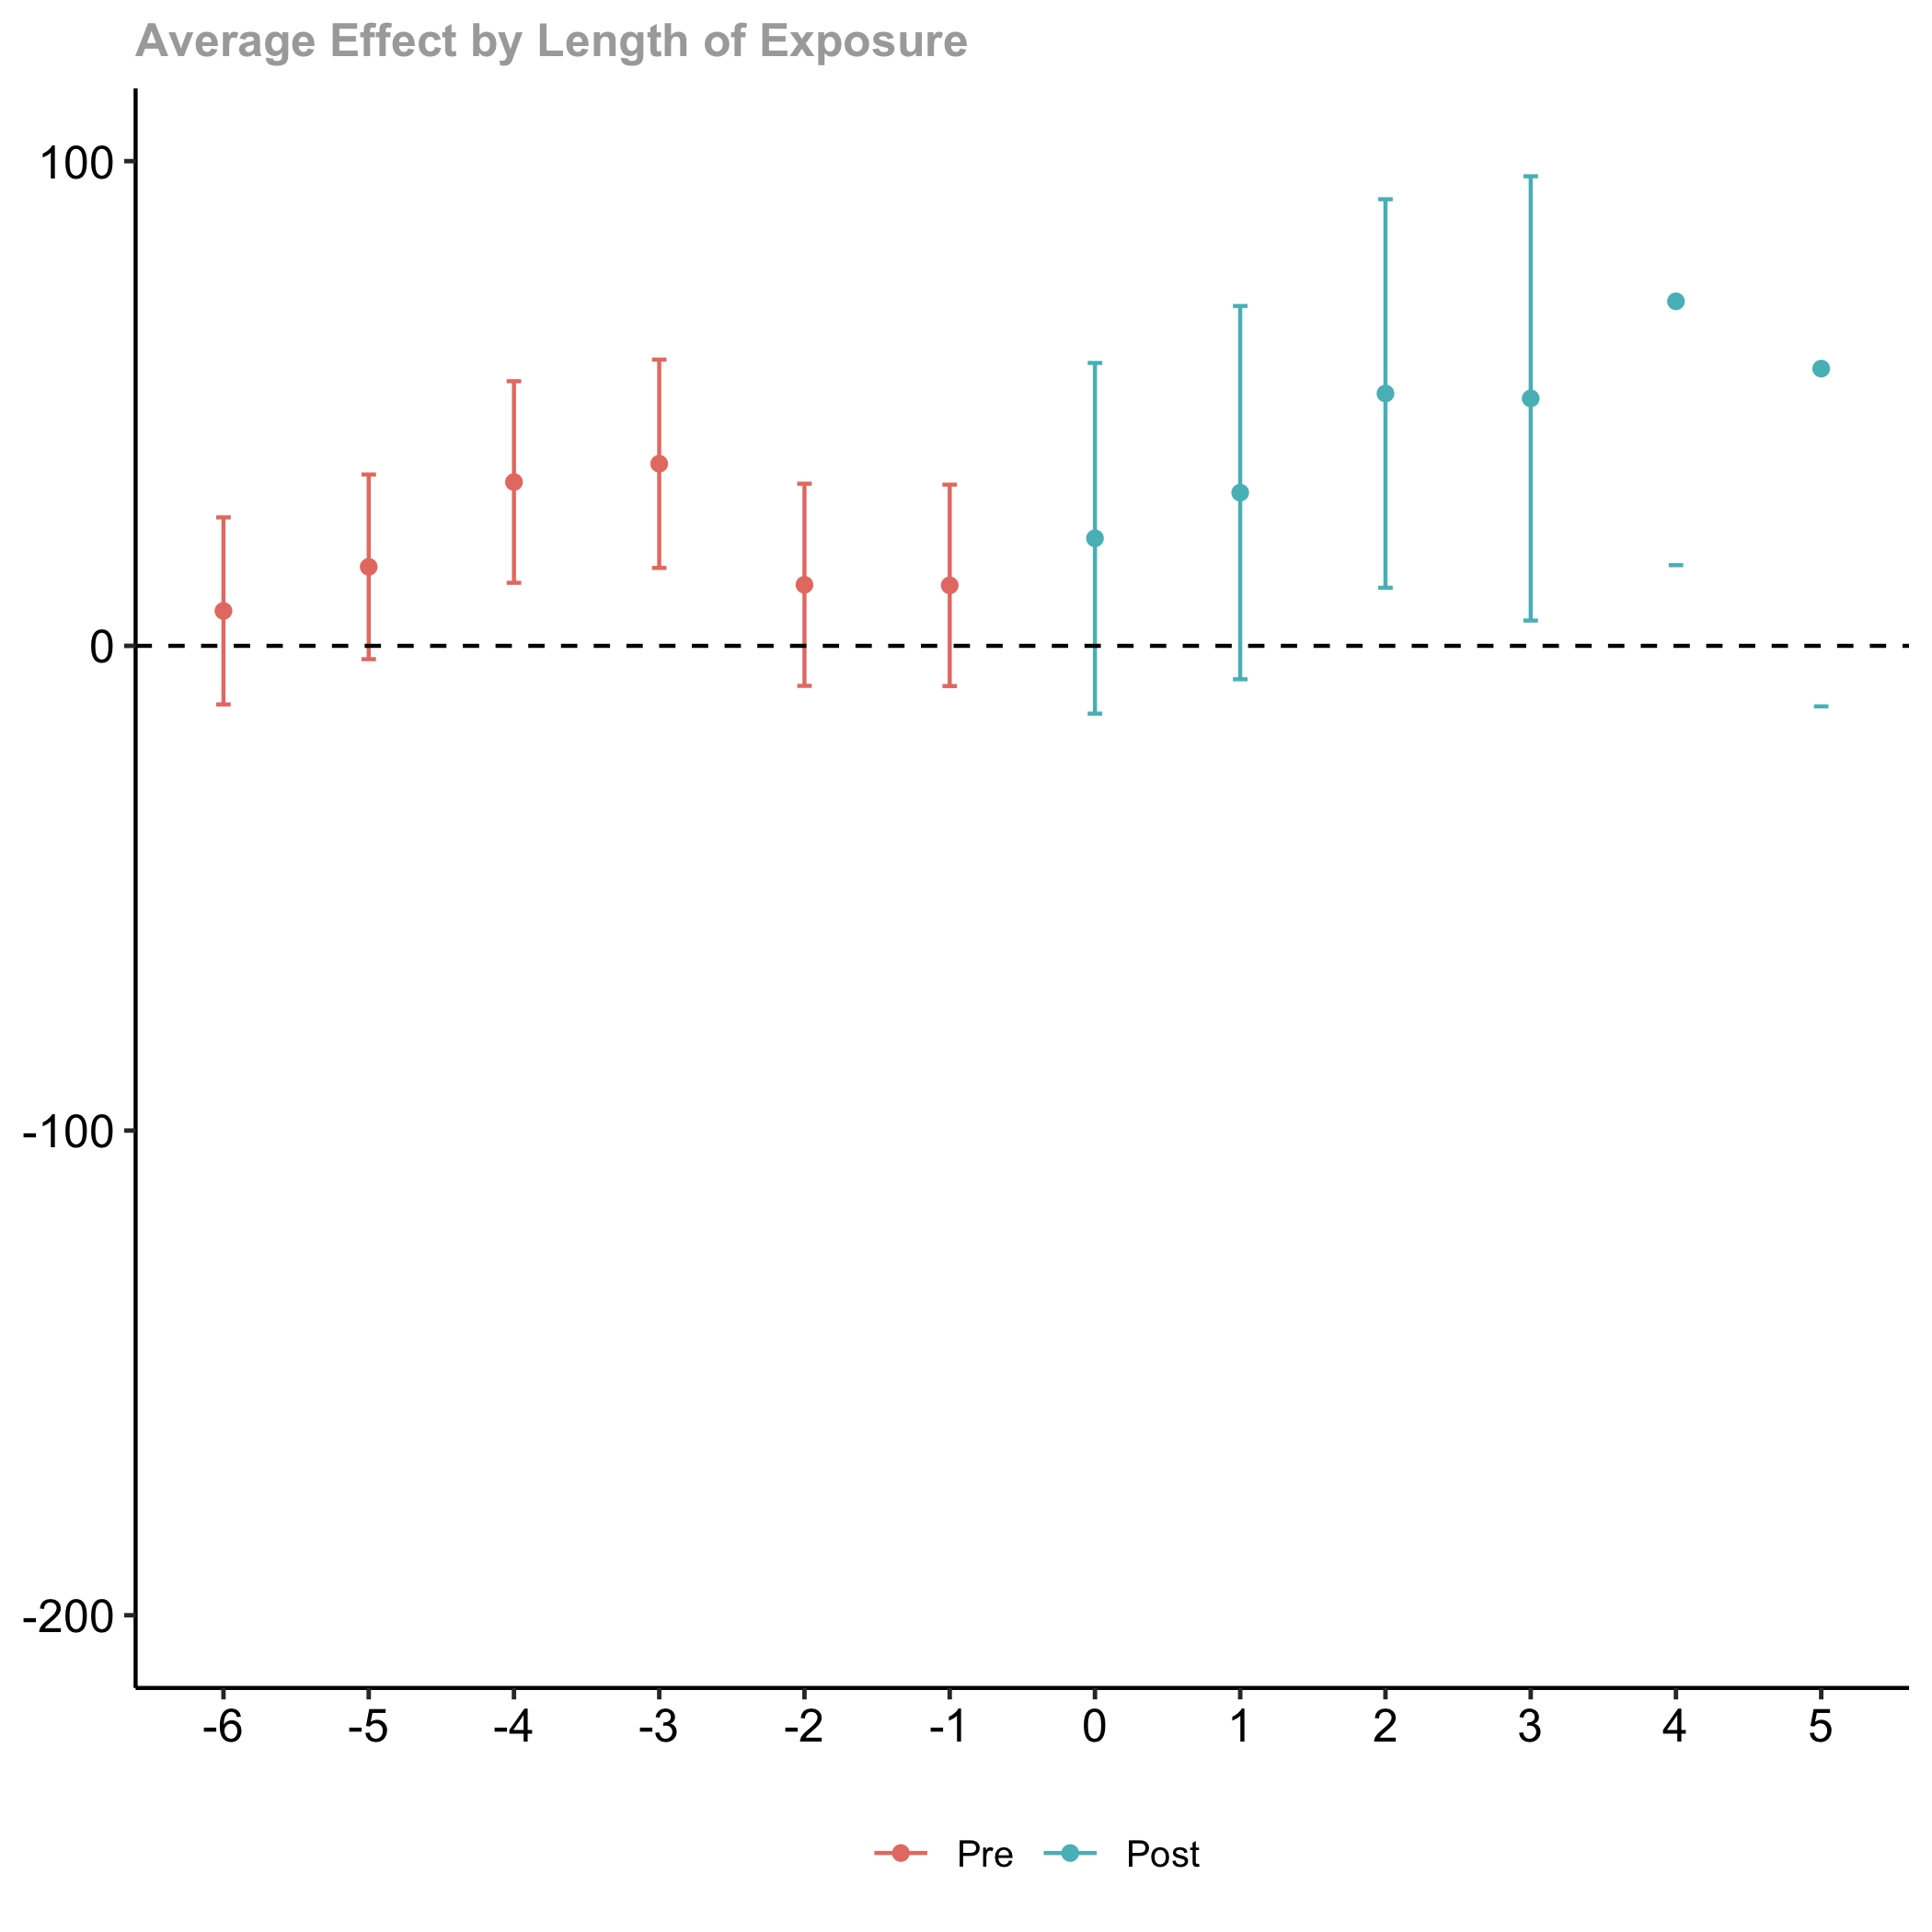
\includegraphics[width=.32\textwidth]{\figdir/antic6_es.png}
    \fignote{\textwidth}{...}
\end{figure}


\subsection{Unbalanced aggregation}%
\label{sub:unbalanced_aggregation}

The baseline specification relies on a panel balanced in event time and
thus only includes groups that have been exposed to treatment for at least 5
periods. Figure~\ref{fig:ub_comp} reproduces the baseline results in the left
panel and compares it with results based on the full sample.

As discussed in \citet{callaway2021difference} (section 3.1.1), these two
approaches entail a trade-off. When using the full sample, the aggregated
parameters are a function of the weighted average treatment effects for each
group $e$ periods after treatment (which is what we want) as well as
compositional changes due to different groups being included for different
periods $e$ and different weights attached to these groups. While parameters
aggregated using a panel balanced in event time do not suffer from
compositional and weighting changes, but are calculated based on a smaller
number of groups.

As expected, using the full data reduces the size of the confidence intervals.
But the results are otherwise very similar.

\begin{figure}[H]
    \centering
    \caption{Comparison of balanced and unbalanced aggregations}%
    \label{fig:ub_comp}
    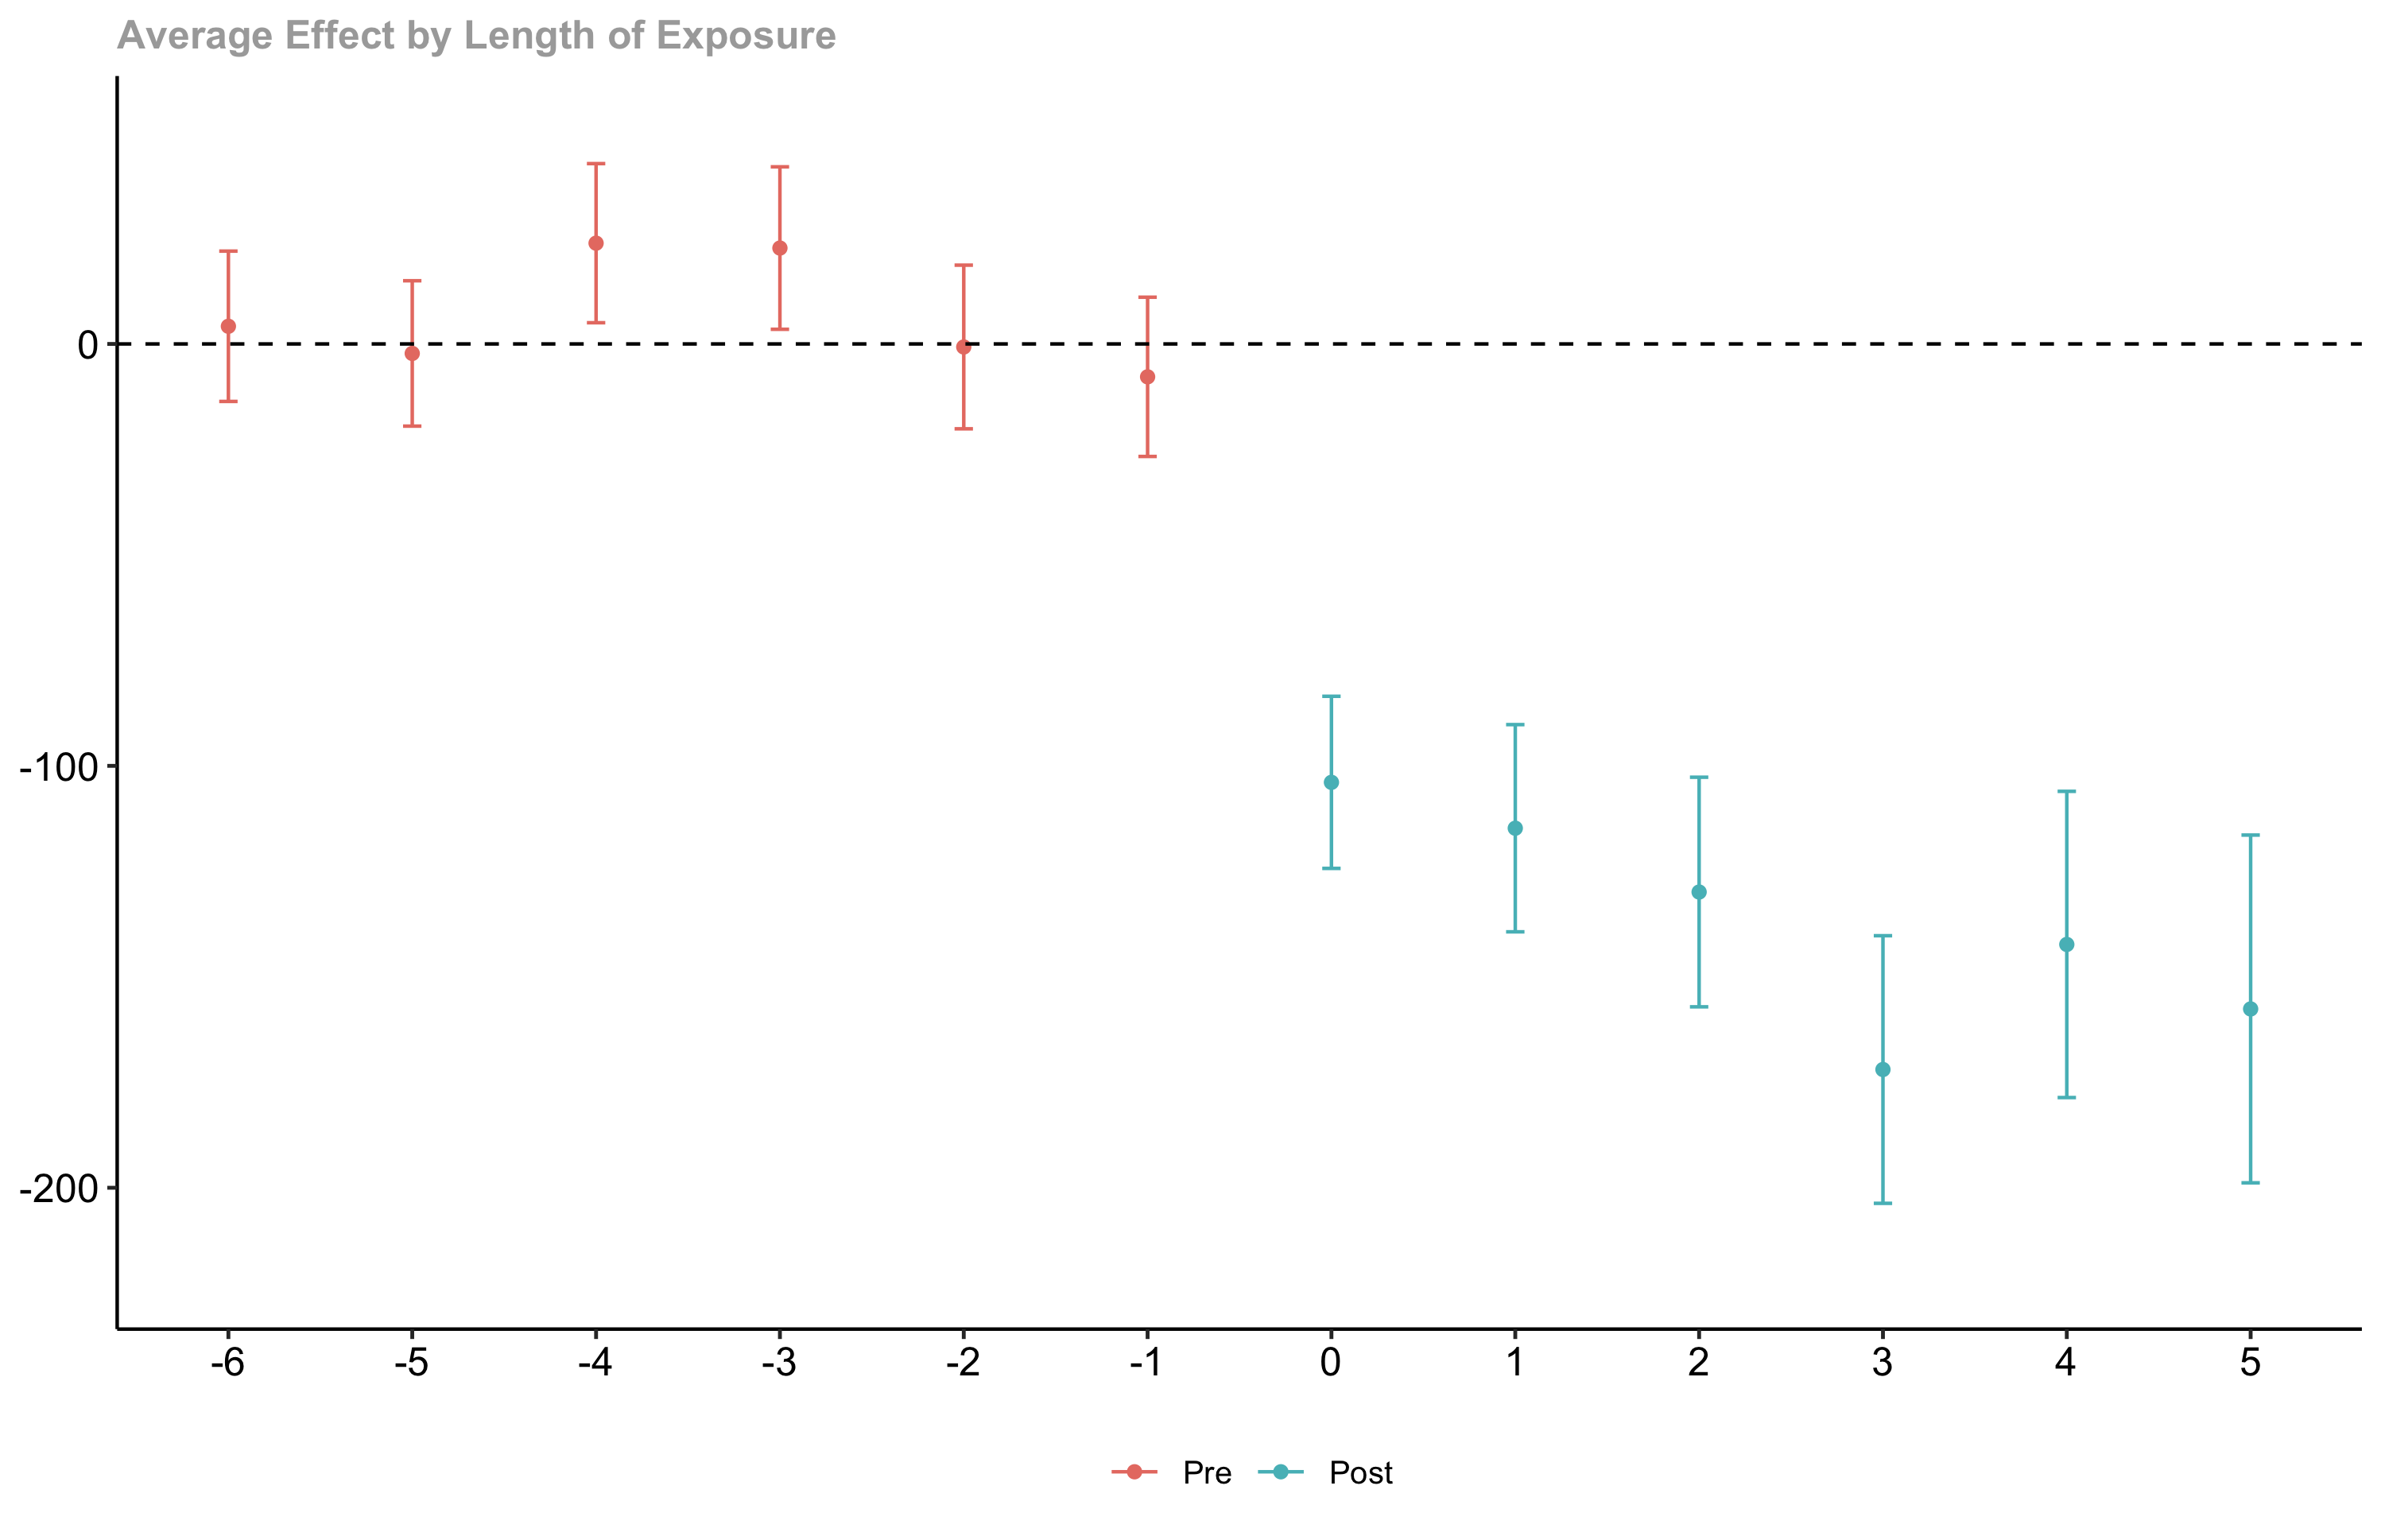
\includegraphics[width=.49\textwidth]{\figdir/bl_es_comp.png}
    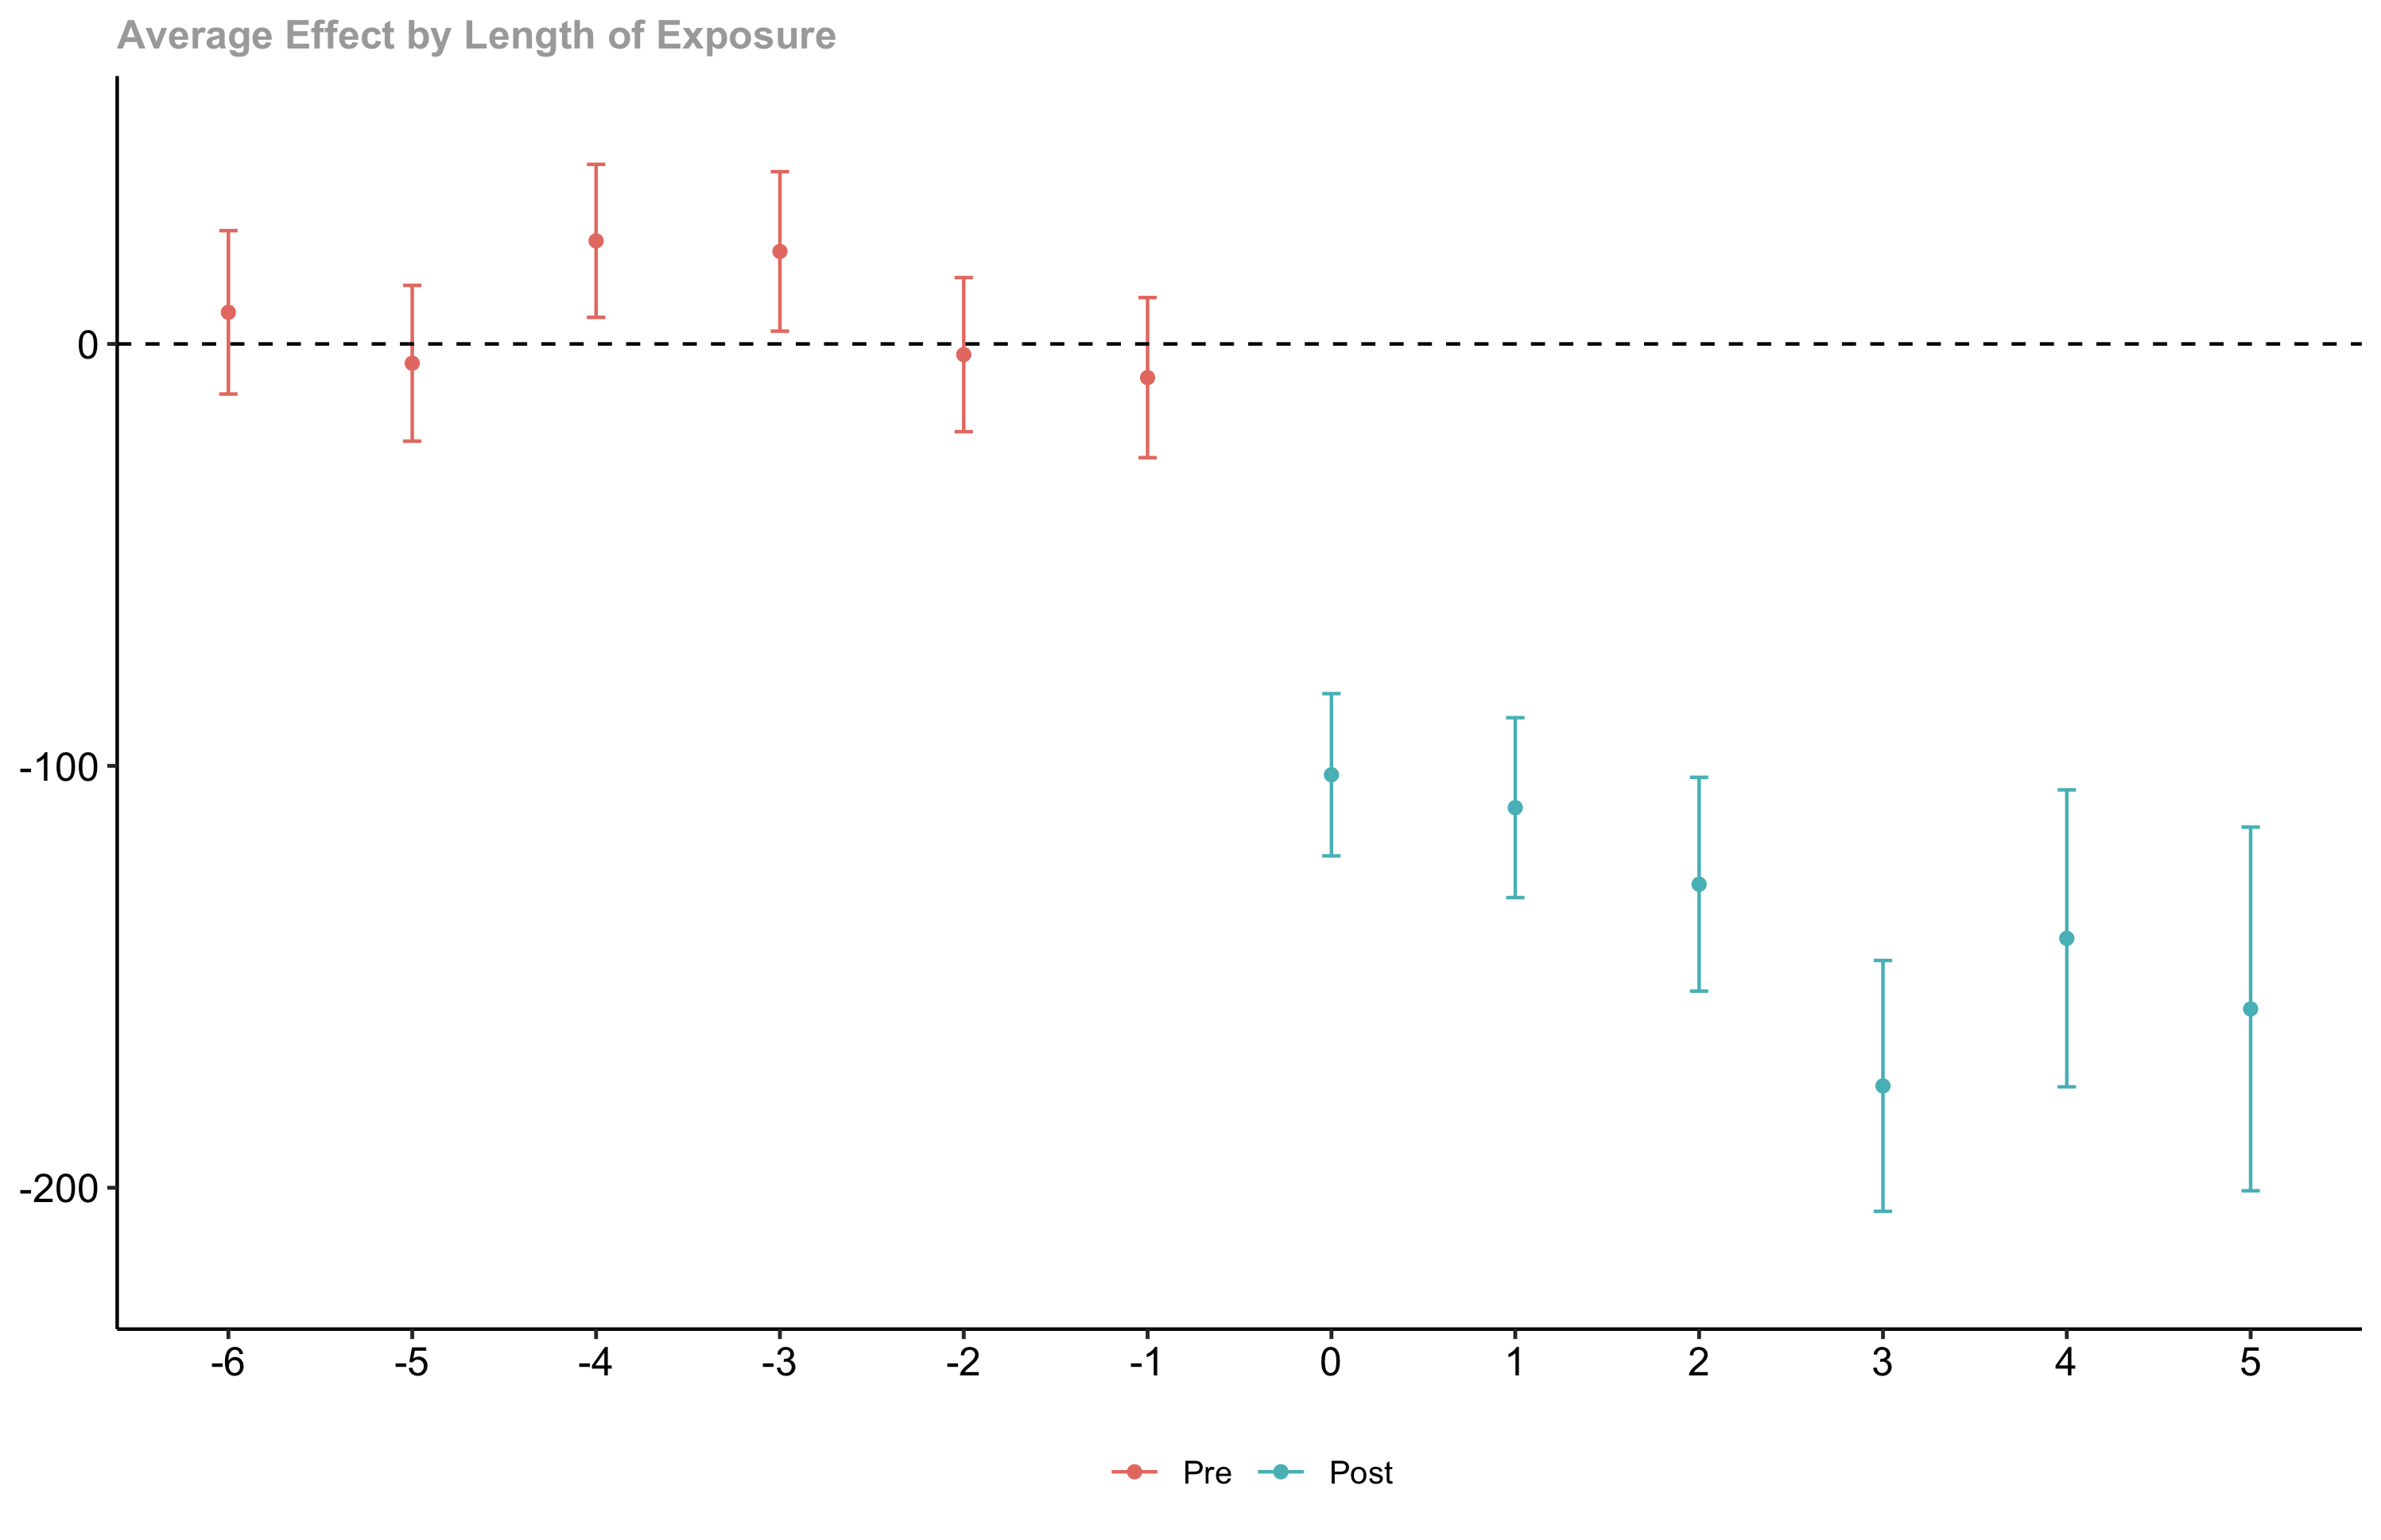
\includegraphics[width=.49\textwidth]{\figdir/ub_es.png}
    \fignote{\textwidth}{...}
\end{figure}




\subsection{Robustness}%
\label{sub:robustness}

\begin{figure}[H]
    \centering
    \caption{New results}%
    \label{fig:new}
    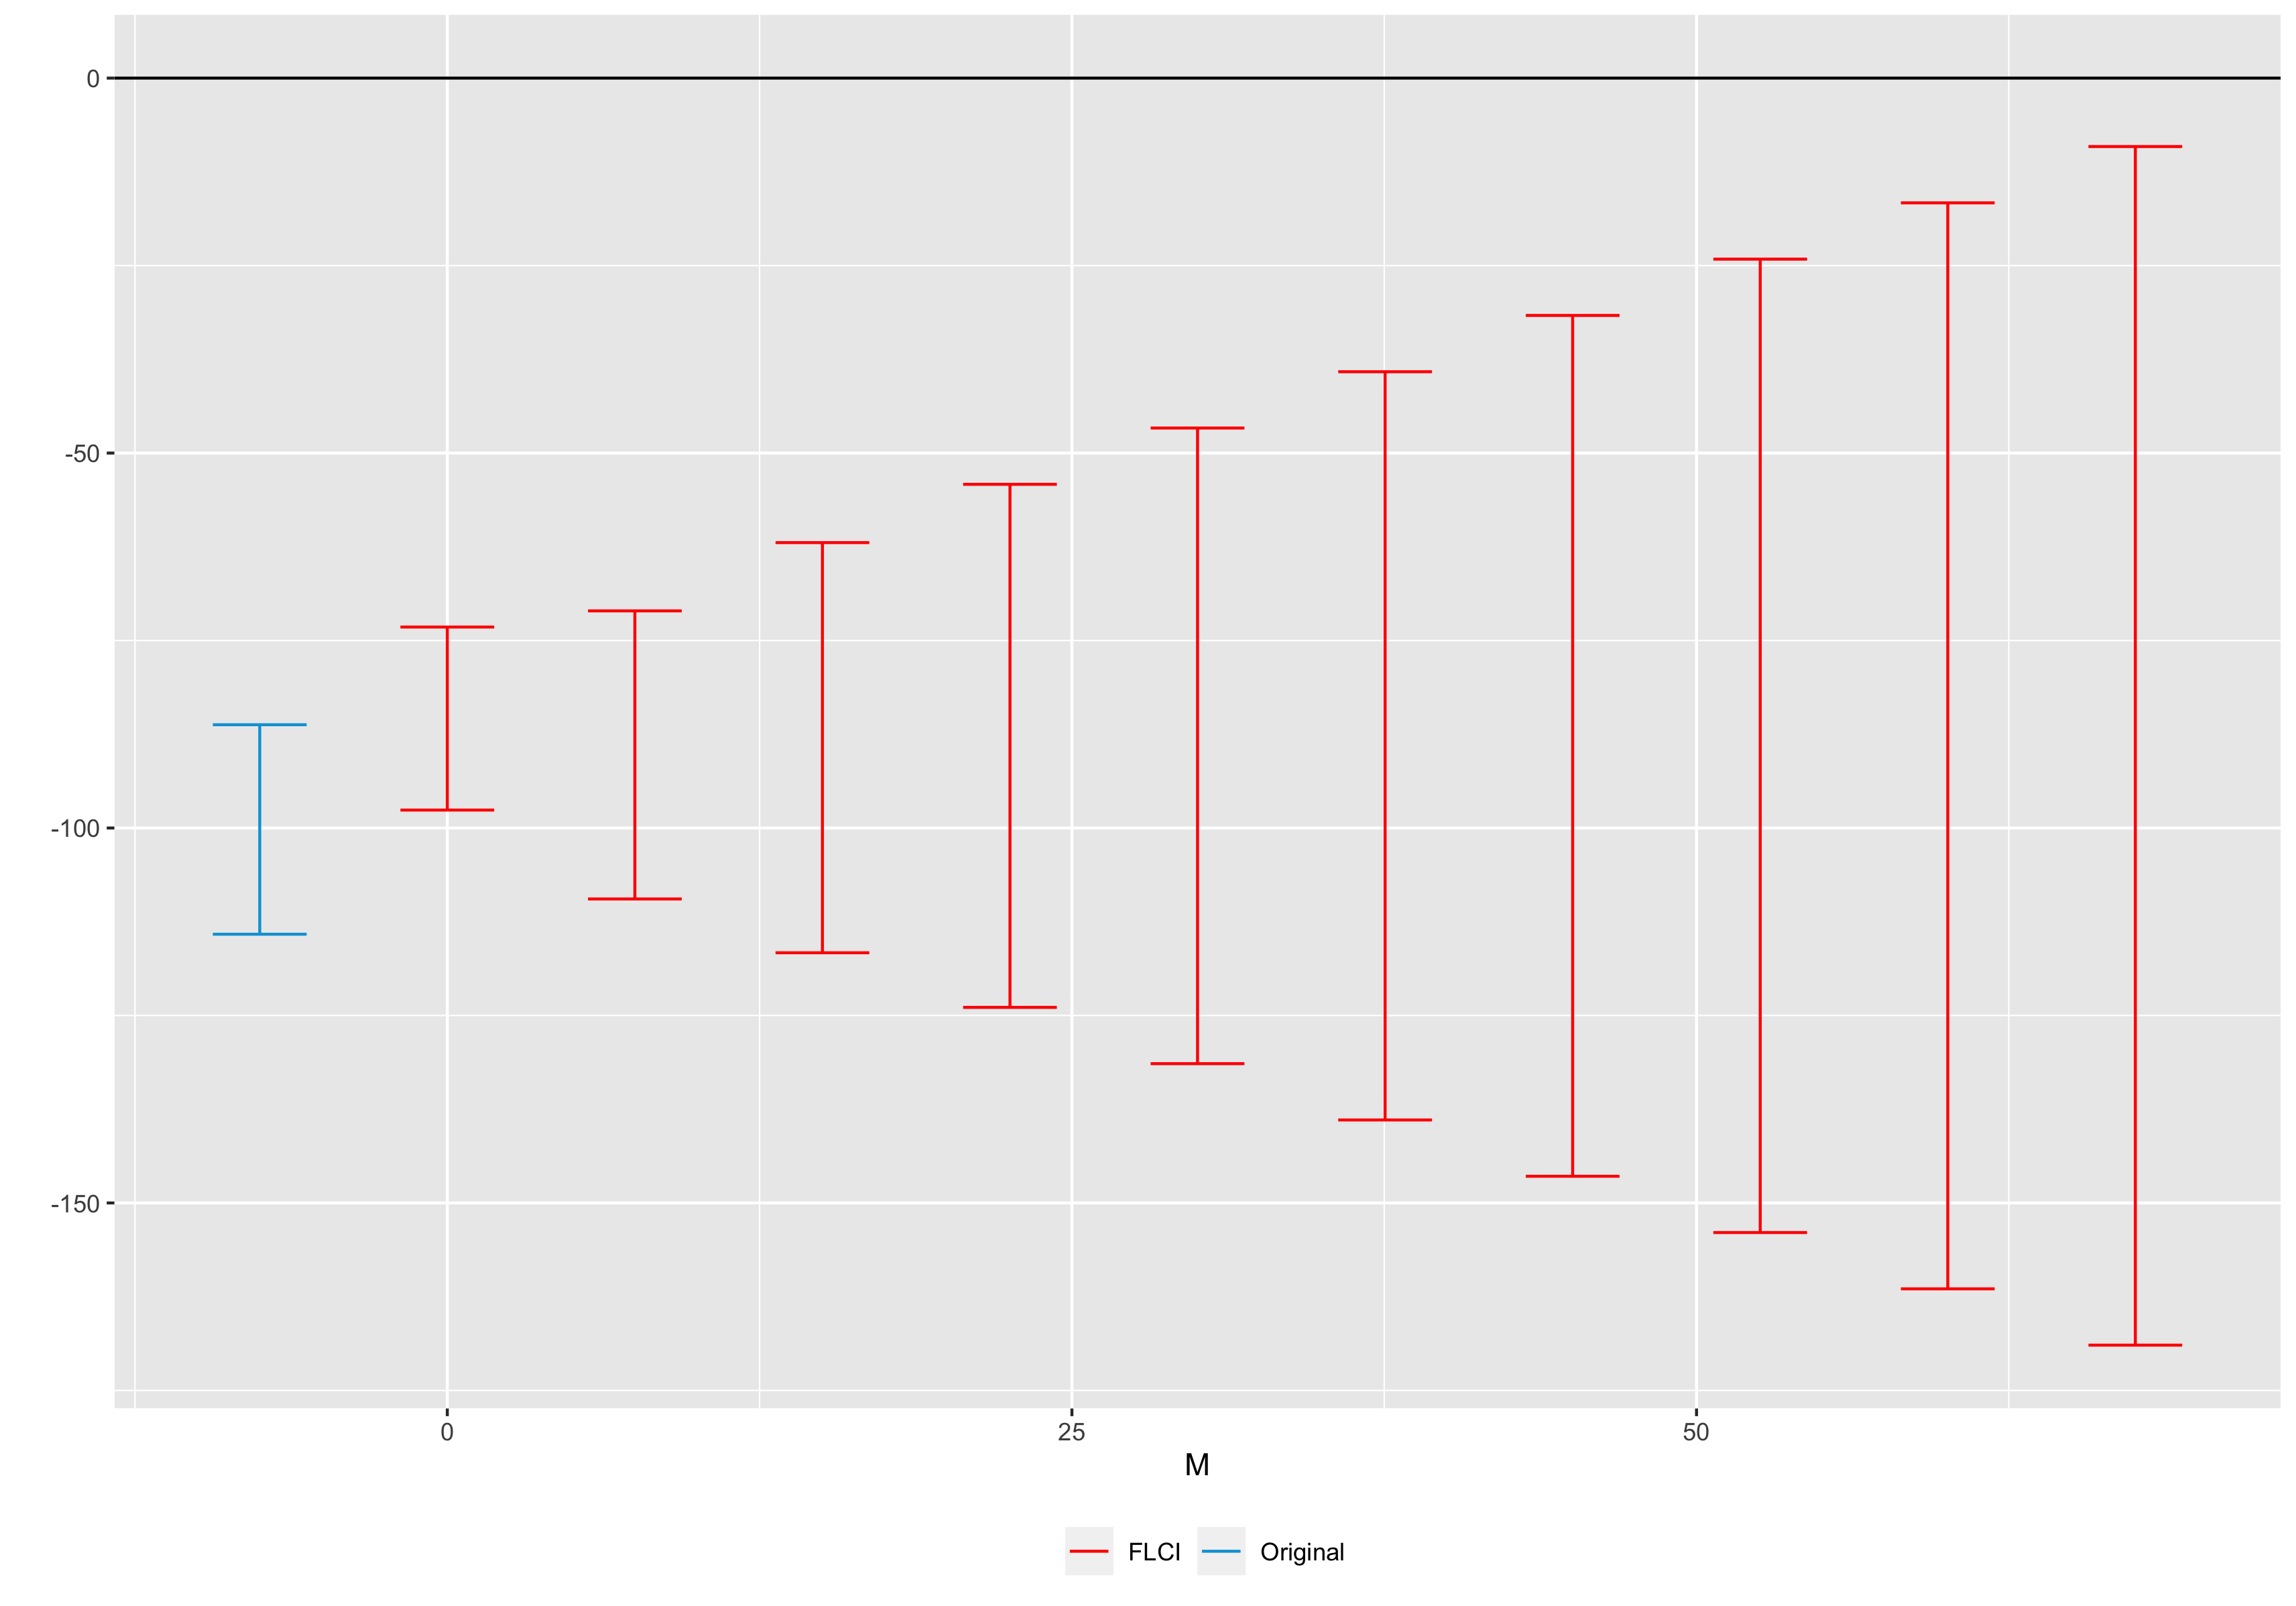
\includegraphics[width=.32\textwidth]{\figdir/cs_hdid_smooth.png}
    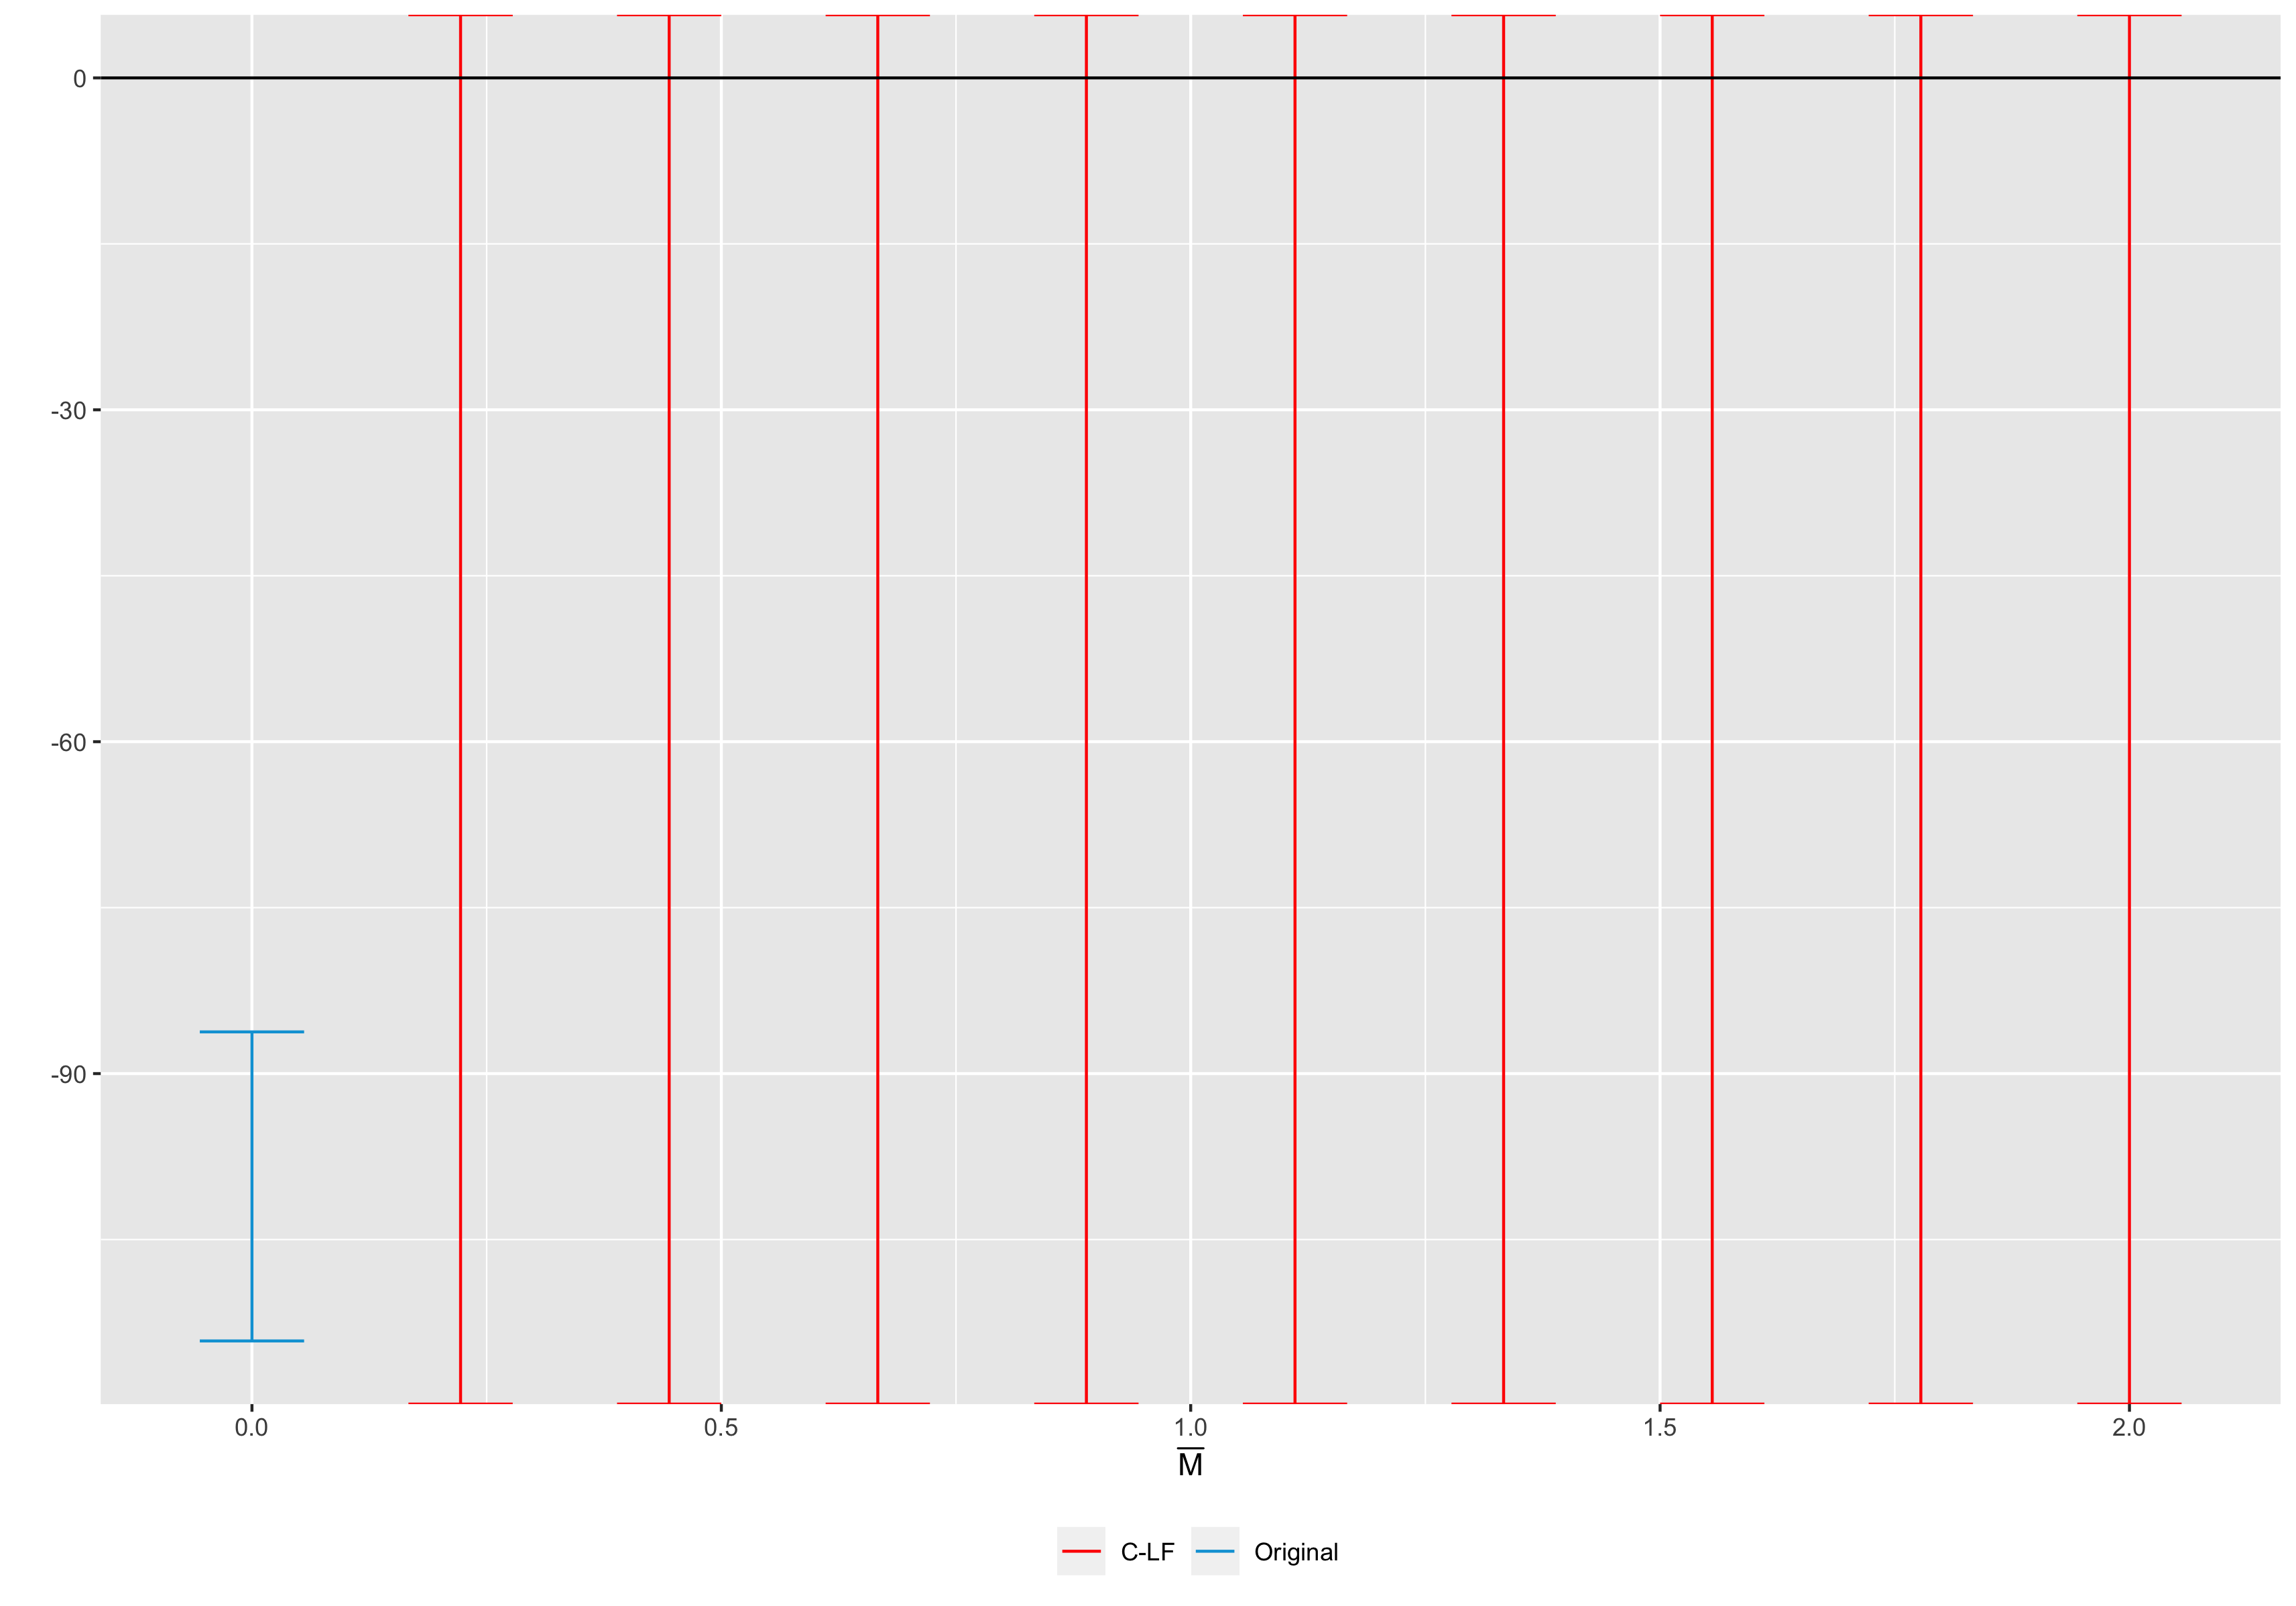
\includegraphics[width=.32\textwidth]{\figdir/cs_hdid_relmag.png}
    \fignote{\textwidth}{...}
\end{figure}











\section{Old stuff}%
\label{sec:old_stuff}











We use an event study design of the following form:

\begin{equation}
\label{eq:dynamic_twfe}
    y_{it} = \sum^{5}_{\substack{s=-6 \\
     s\neq-1}} \beta_s D_{it}^s + \alpha_i + \lambda_t + \gamma X_{it} + \epsilon_{it},
\end{equation}

where $y_{it}$ is the outcome for individual $i$ at time $t$, $\alpha_i$ and
$\lambda_t$ are individual and year-month fixed effects, respectively, and
$X_{it}$ is a vector of individual and time varying controls. $D_{it}^s$ equals
1 if, in period $t$, individual $i$ is $s$ months away from signing up to the
app. The set of $\beta_s$ coefficients measure the effect of treatment $s$
periods away from treatment, which is what we are interested in.

We normalise our treatment effects by expressing them relative to reference
period $s = -1$, which is necessary to avoid perfect multicollinearity between
the relative period indicators (which sum to 1 for each user-month observation)
and the user-level fixed effect $alpha_i$ (which also equals 1). We follow
common practice and normalise relative to the last period before treatment
exposure because this serves as a natural benchmark for post-treatment
behaviour.

To avoid multicollinearity issues and uniquely identify the lead and lag
effects, we omit relative period indicator $s = -1$,

and bin the endpoints of our observation window so that $D_{it}^{-6} = 1$ for
all periods six or more periods prior to signup and $D_{it}^{5} = 1$ for all
months five or more months after the month of signup. We choose a window from
-6 to 5 for two reasons: because the longer a window we consider, the less
plausible our ceteris paribus assumption is, and the longer the window, the
smaller our sample.


Normalising: 

This expresses all estimates relative to the omitted
period, which -- given that it is the last month before signup -- serves as a
natural benchmark.

% We omit the relative period indicator for period $s = -1$ because we need to
% omit one relative period indicator to avoid perfect collinearity among the
% period indicators, and we choose the last pre-treatment period because it
% serves as a natural benchmark against which to compare the outcomes in other
% periods.\footnote{As \citet{sun2021estimating} point out, there are two sources
% of perfect multicollinearity when estimating a fully dynamic model (i.e. one
% including all possible lags). The first results from all relative period
% indicators summing to 1 in each period, so that the entire set of relative period
% dummies across all time periods is perfectly multicollinear. We deal with this
% by excluding the indicator for $s = -1$. The second issue arises from the fact
% that for initial treatment period $E_i$, $t = s + E_i$. We deal with this issue
% by "trimming" our sample to be balanced in relative periods by only using
% data from relative periodl $\{-6, 5\}$. Both of these approaches are standard
% in the empirical literature.}


Binning:
Binning endpoints assumes that coefficients remain constant
outside the observation window.

Both of these approaches are standard in the
literature, as discussed in \citet{sun2021estimating, schmidheiny2019event}.

Assumptions:
\begin{itemize}
    \item Homogenous treatment paths across cohorts.

    \item Strict exogeneity of treatment assumption doesn't hold due to
        self-selection into app use. Consequence: can't estimate causal effect
        of app use.
\end{itemize}

Notes:
\begin{itemize}
    \item \citet{sun2021estimating} show that event study design is fine even
        in the presence of no untreated units, as long as dynamic trajectory of
        effect is the same for all cohorts.

    \item 
\end{itemize}

Time fixed effects:
\begin{itemize}
    \item Using ym vs m.
\end{itemize}


\begin{figure}[H]
    \centering
    \caption{Main results}%
    \label{fig:dspend_main}
    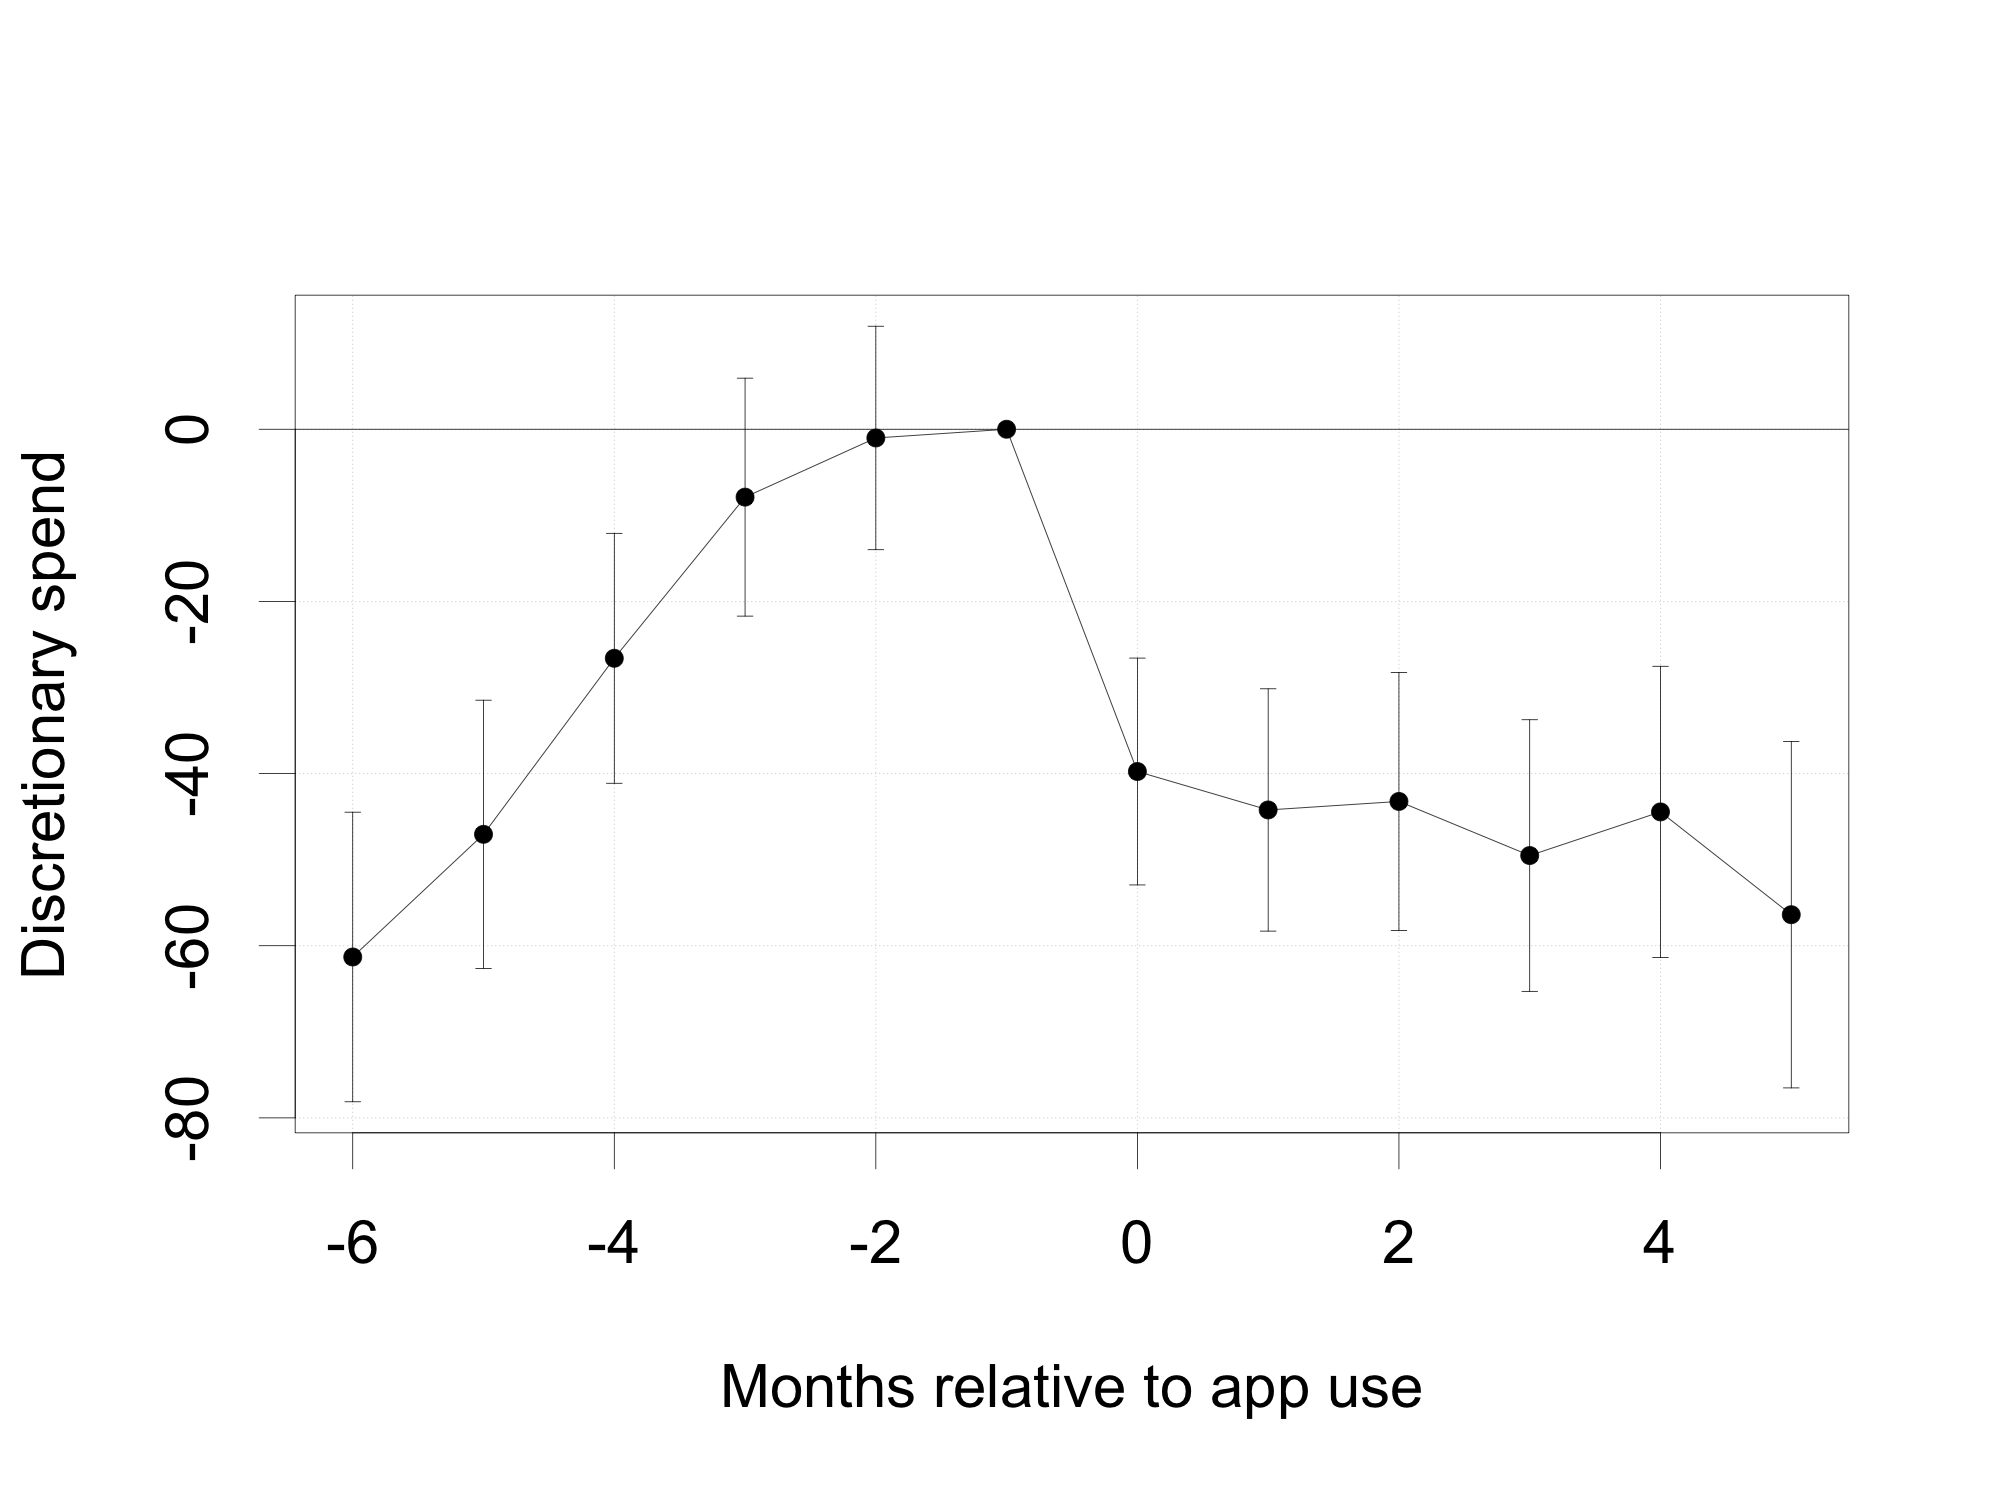
\includegraphics[width=.49\textwidth]{\figdir/dspend_main.png}
    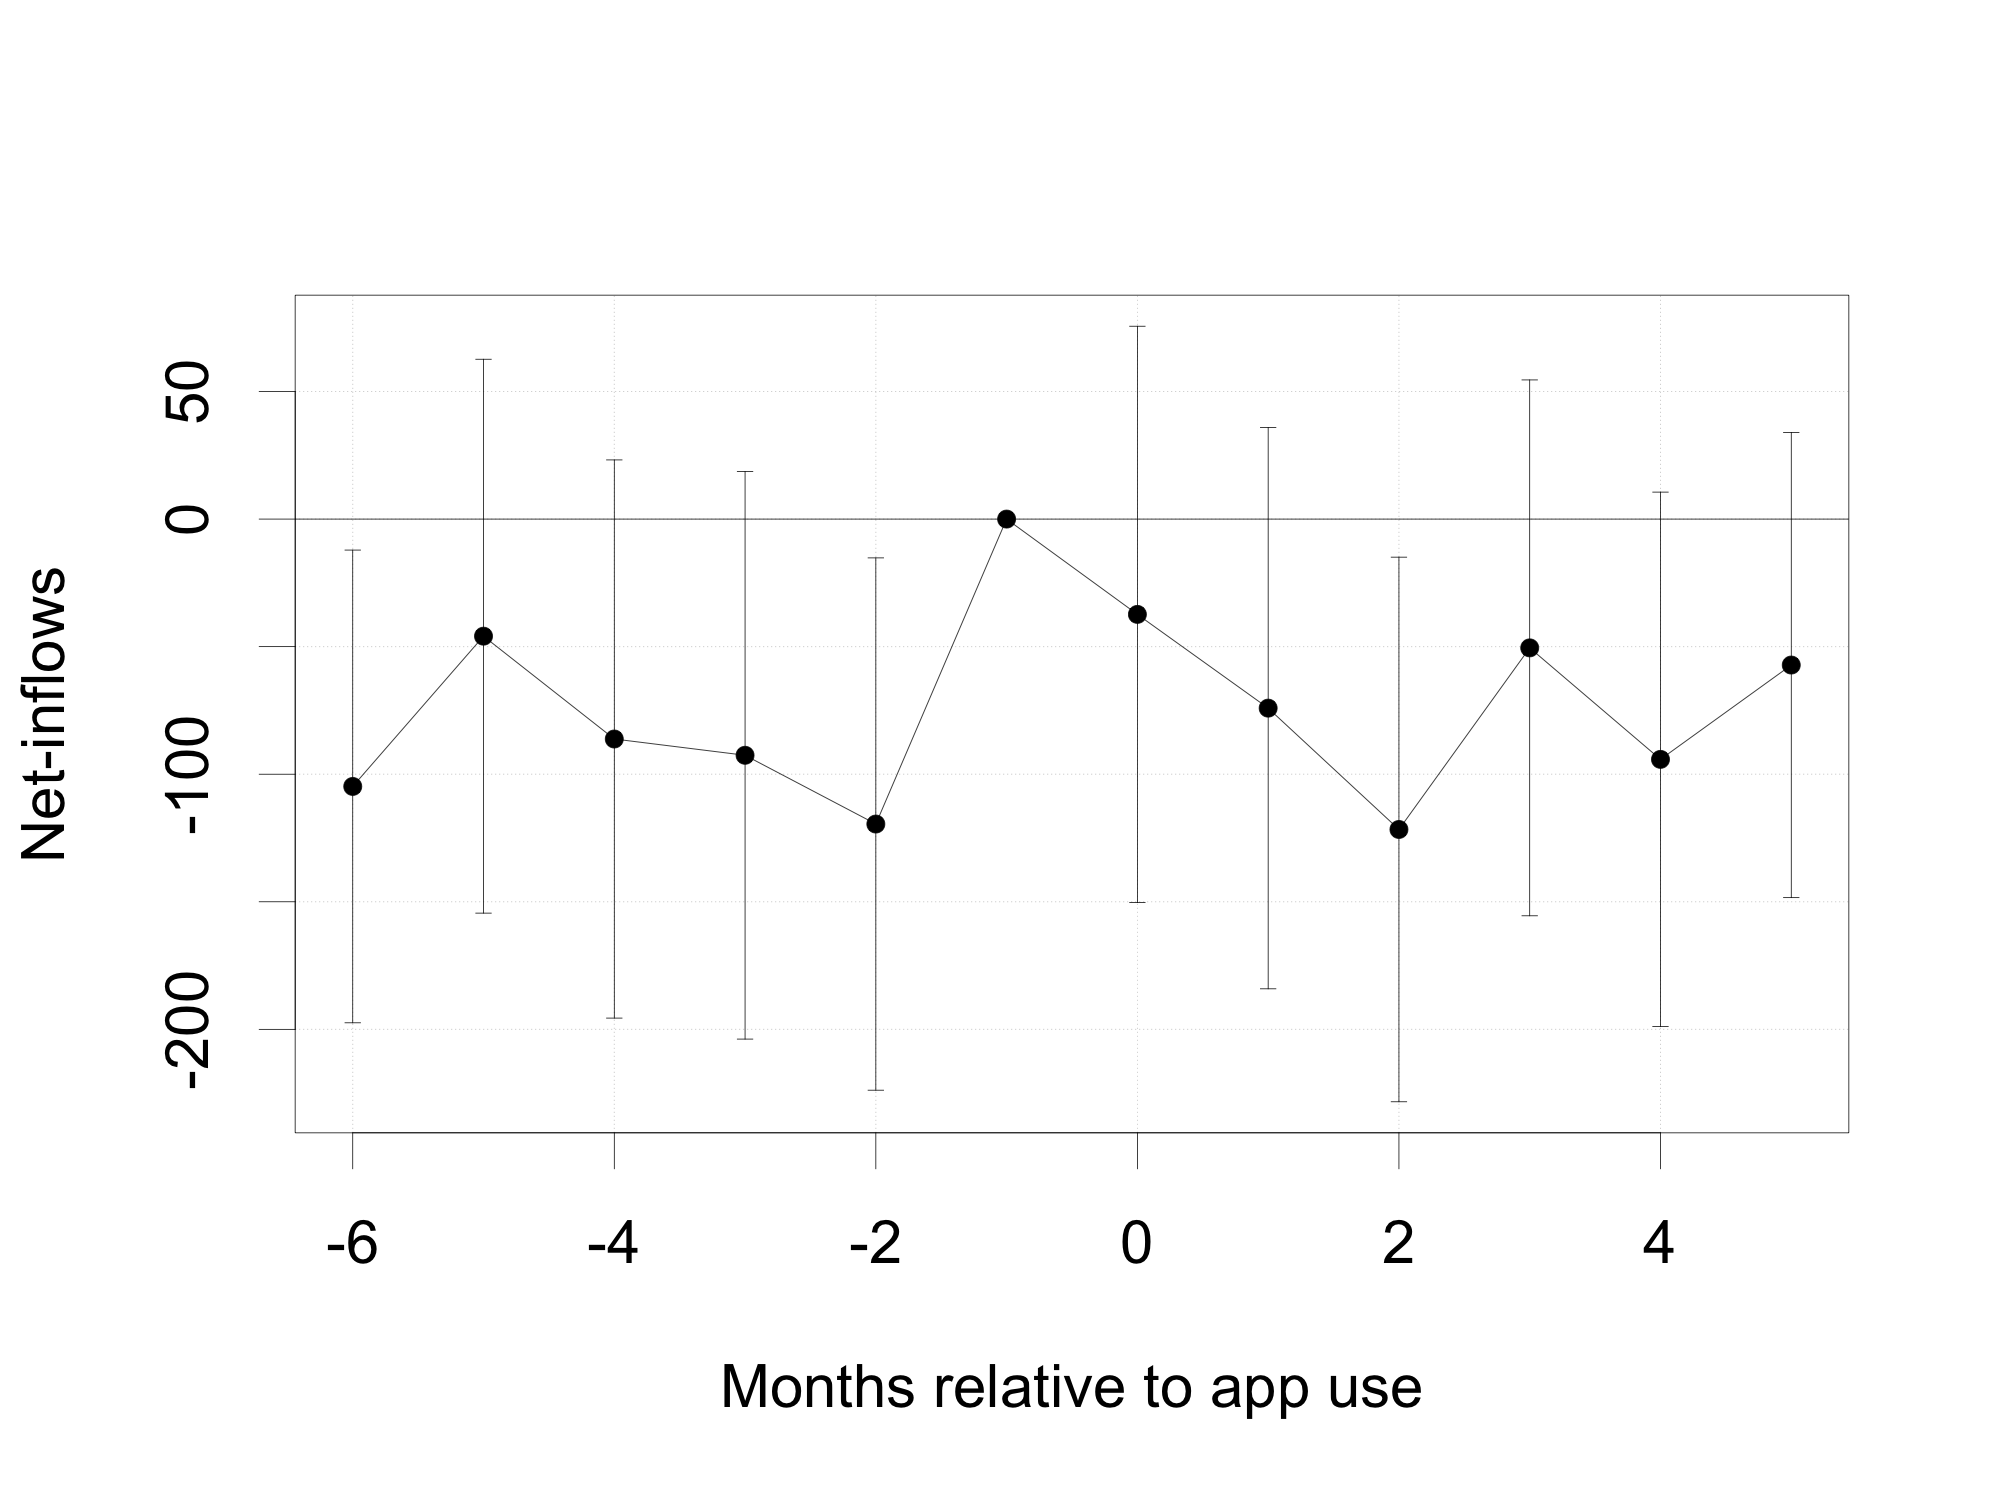
\includegraphics[width=.49\textwidth]{\figdir/netflows_main.png}
    \fignote{\textwidth}{Figures show estimates of leads and lags frome
        estimating model~(\ref{eq:dynamic_twfe}) with distretionary spend (left) and
netflows into savings accounts (right) as the dependent variable. Standard
errors are clustered by user.}
\end{figure}





% \citet{sun2021estimating} define an event study design as a staggered adoption
% design where units are treated at different times and where there may or may
% not be never treated units. In our case, we have no never treated units, and
% treatment is absorbing in that once a unit is treated they will also be treated
% in all subsequent units.\footnote{We cannot rule out that some users who
% stopped using the app and closed their account rejoined later on, in which case
% they would appear in our dataset as a new user. However, we can plausibly
% assume that such cases are rare.} 

% Setup:
% \begin{itemize}
%     \item We observe $N+1$ unites for $T+1$ periods and, for each
%         $i\in\{0,\ldots, N\}$ and $t\in\{0,\ldots,T\}$ observe outcome $y_{it}$
%         and treatment status $D_{it}\in\{0, 1\}$, where $D_{it}$ equals 1 if unit
%         $i$ is treated in period $t$ and 0 otherwise.

%     \item We can uniquely characterise treatment paths by the time period of
%         initial treatment, denoted as $E_i = min\{t: D_{it} = 1\}$.

%     \item We can group units into cohorts $e \in \{0,\ldots, T\}$, where units
%         in cohort $e$ were all first treated at time $e$, so that $\{i: E_i =
%         e\}$.

%     \item We define $y^e_{it}$ as the potential outcome in period $t$ if unit
%         $i$ was first treated in period $e$.

% \end{itemize}


% Assumptions:
% \begin{itemize}
%     \item Observations $\{y_{it}, D_{it}\}_{t=0}^T$ are independent.

%     \item A1: parallel trends: difference in baseline outcomes over time do
%         not differ between treatment cohorts. Not obviously violated in our
%         context. Early adopters might differ from late adopters, but difference
%         might plausibly be constant over time. - We don't have never treated
%         units, so Ashenfelter dip scenario is not a problem, even though we
%         seem to observe something like this in discretionary spending graph
%         (increase in disc spend before signup)

%     \item A2: no anticipatory behaviour. Plausibly violated if people are
%         motivated to save more and start doing so even before app use. Can test
%         for whether there is a peak prior to signup. Because our units have
%         private knowledge about future of treatment path (their intention to
%         reduce spending and save more and sign up to an app), this might be
%         violated. The trajectories of discret spend and net inflows are
%         conflicting on this, though, suggesting that they increases discret
%         spend in runup to app use (which might provide motivation to eventually
%         sign up) but also might have increased net savings slightly.

%     \item A3: treatment effect homogeneity across all cohorts and all relative
%         periods. (Note: treatment effects can be dynamic, but need to be the
%         same across cohorts). We could test for this.

% \end{itemize}


% Notes:
% \begin{itemize}

%     \item Comparison: pre vs post signup within each individual.

%     \item Assumption: there are no time-varying unobserved effects that affect
%         both y and D (formally: $E[Du] = 0$, since u is by definition
%         correlated with y.

%     \item Discussion: there is something that made the individual sign up in
%         the first place, and it might well be an individual level shock that we
%         don't observe (unexpected large expense, loss of job, exposure to
%         something that motivates saving or change in financial behaviour).

%     \item See \citet{imai2021use} for problems with twfe

% \end{itemize}



\subsection{Decomposing intensive and extensive margins}%
\label{sub:decomposing_intensive_and_extensive_margins}
\begin{figure}[H]
    \centering
    \caption{Decomposition of intensive and extensive margins}%
    \label{fig:intext}
    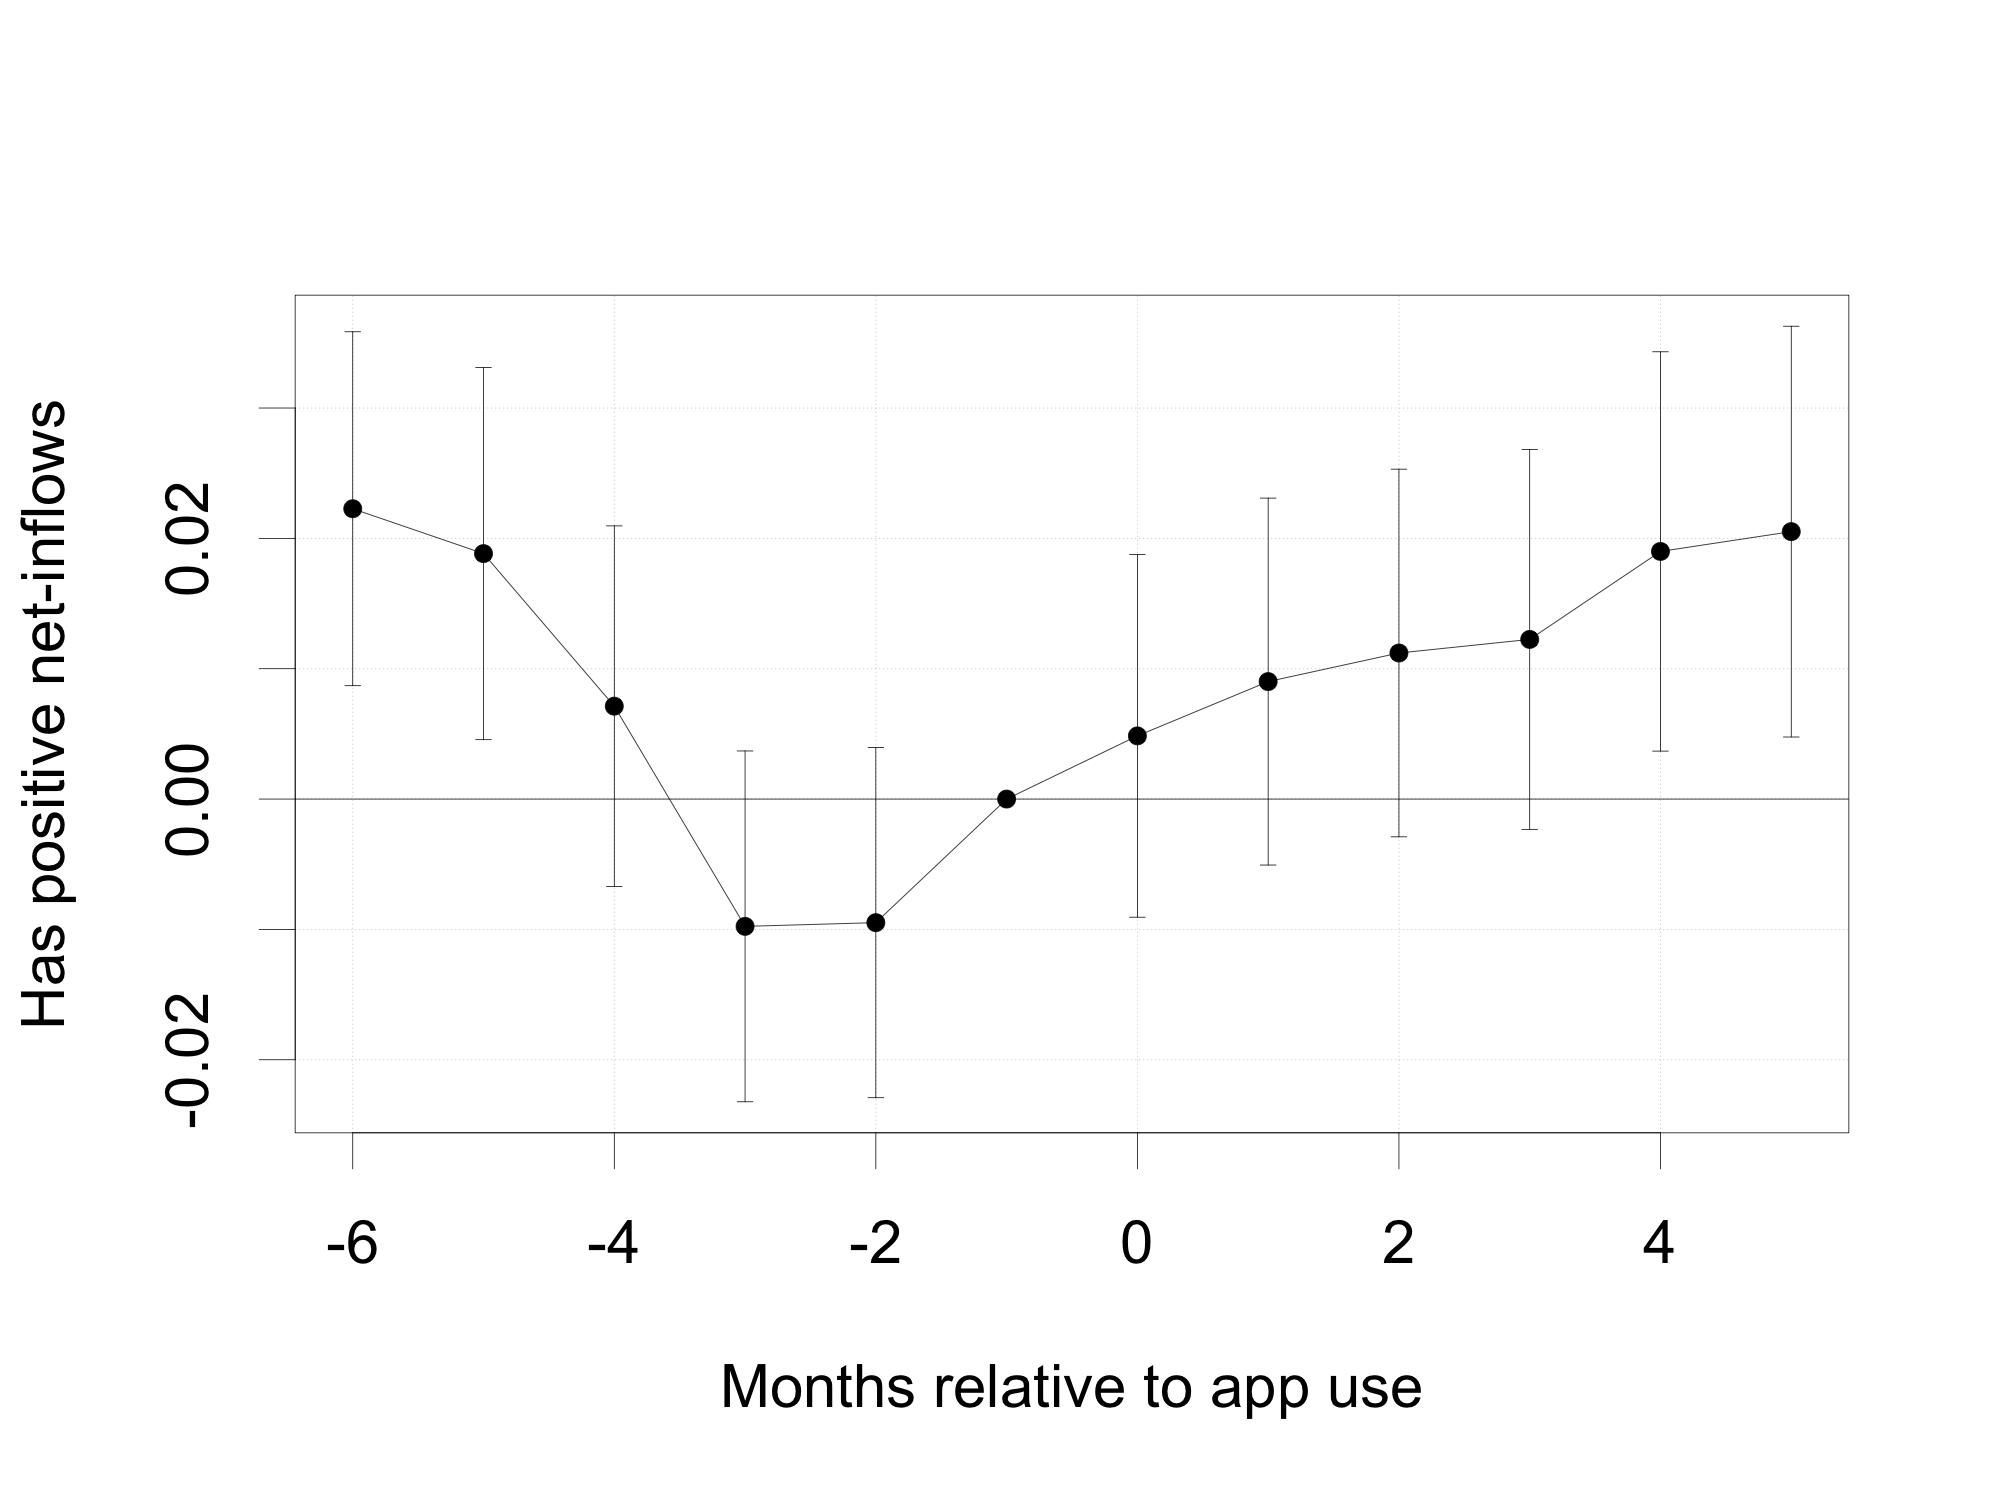
\includegraphics[width=.49\textwidth]{\figdir/has_pos_netflows.png}
    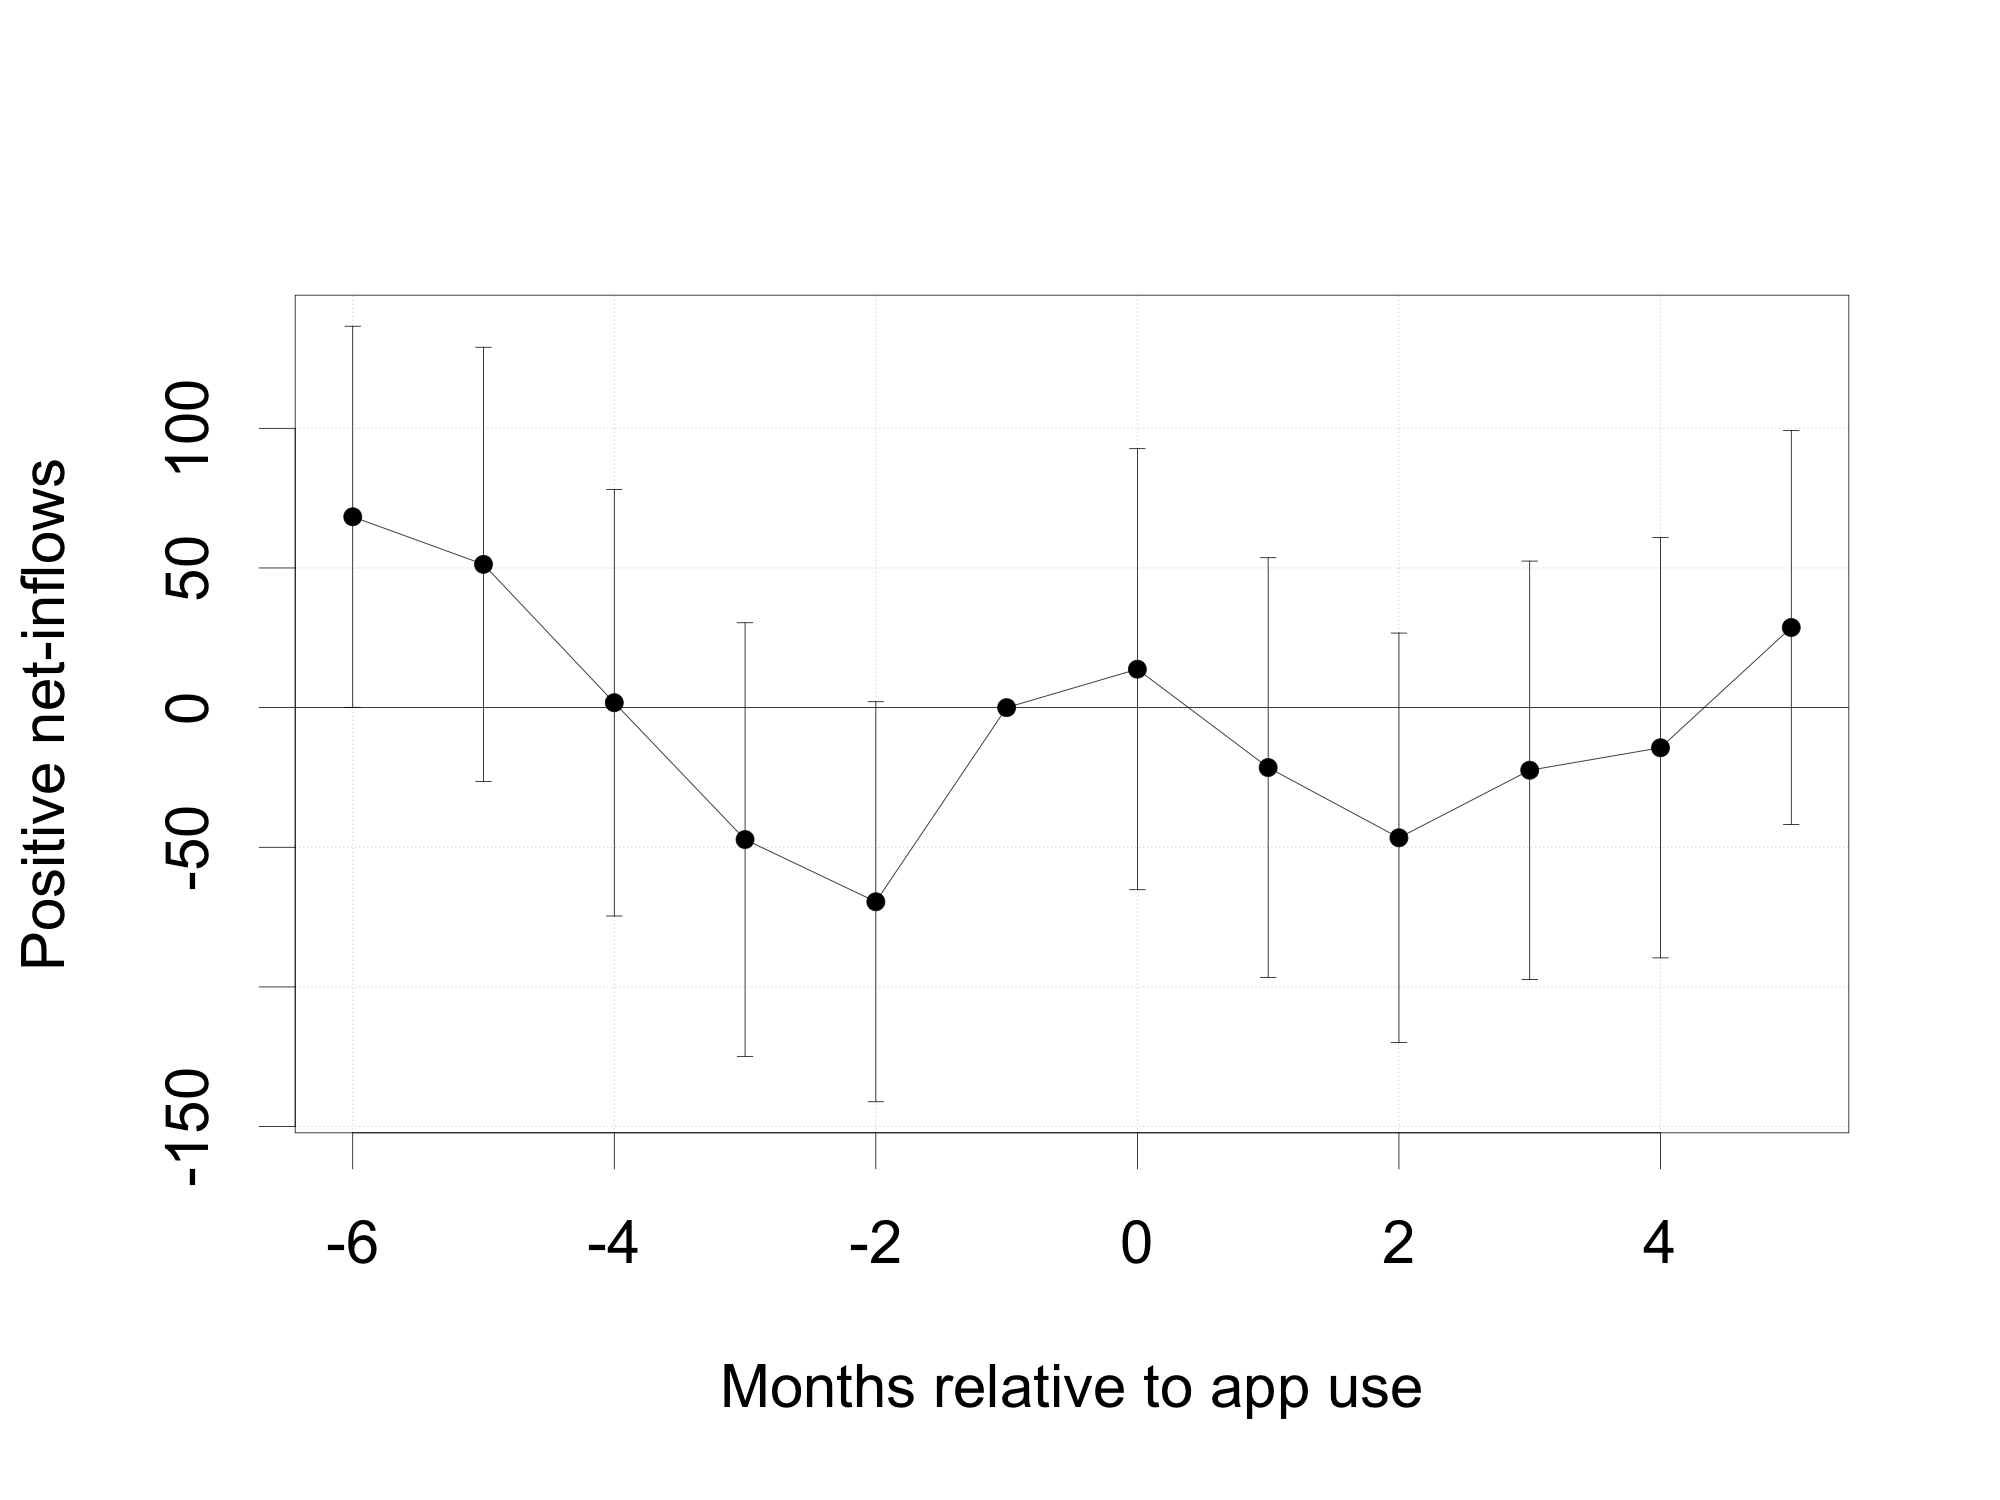
\includegraphics[width=.49\textwidth]{\figdir/pos_netflows.png}
    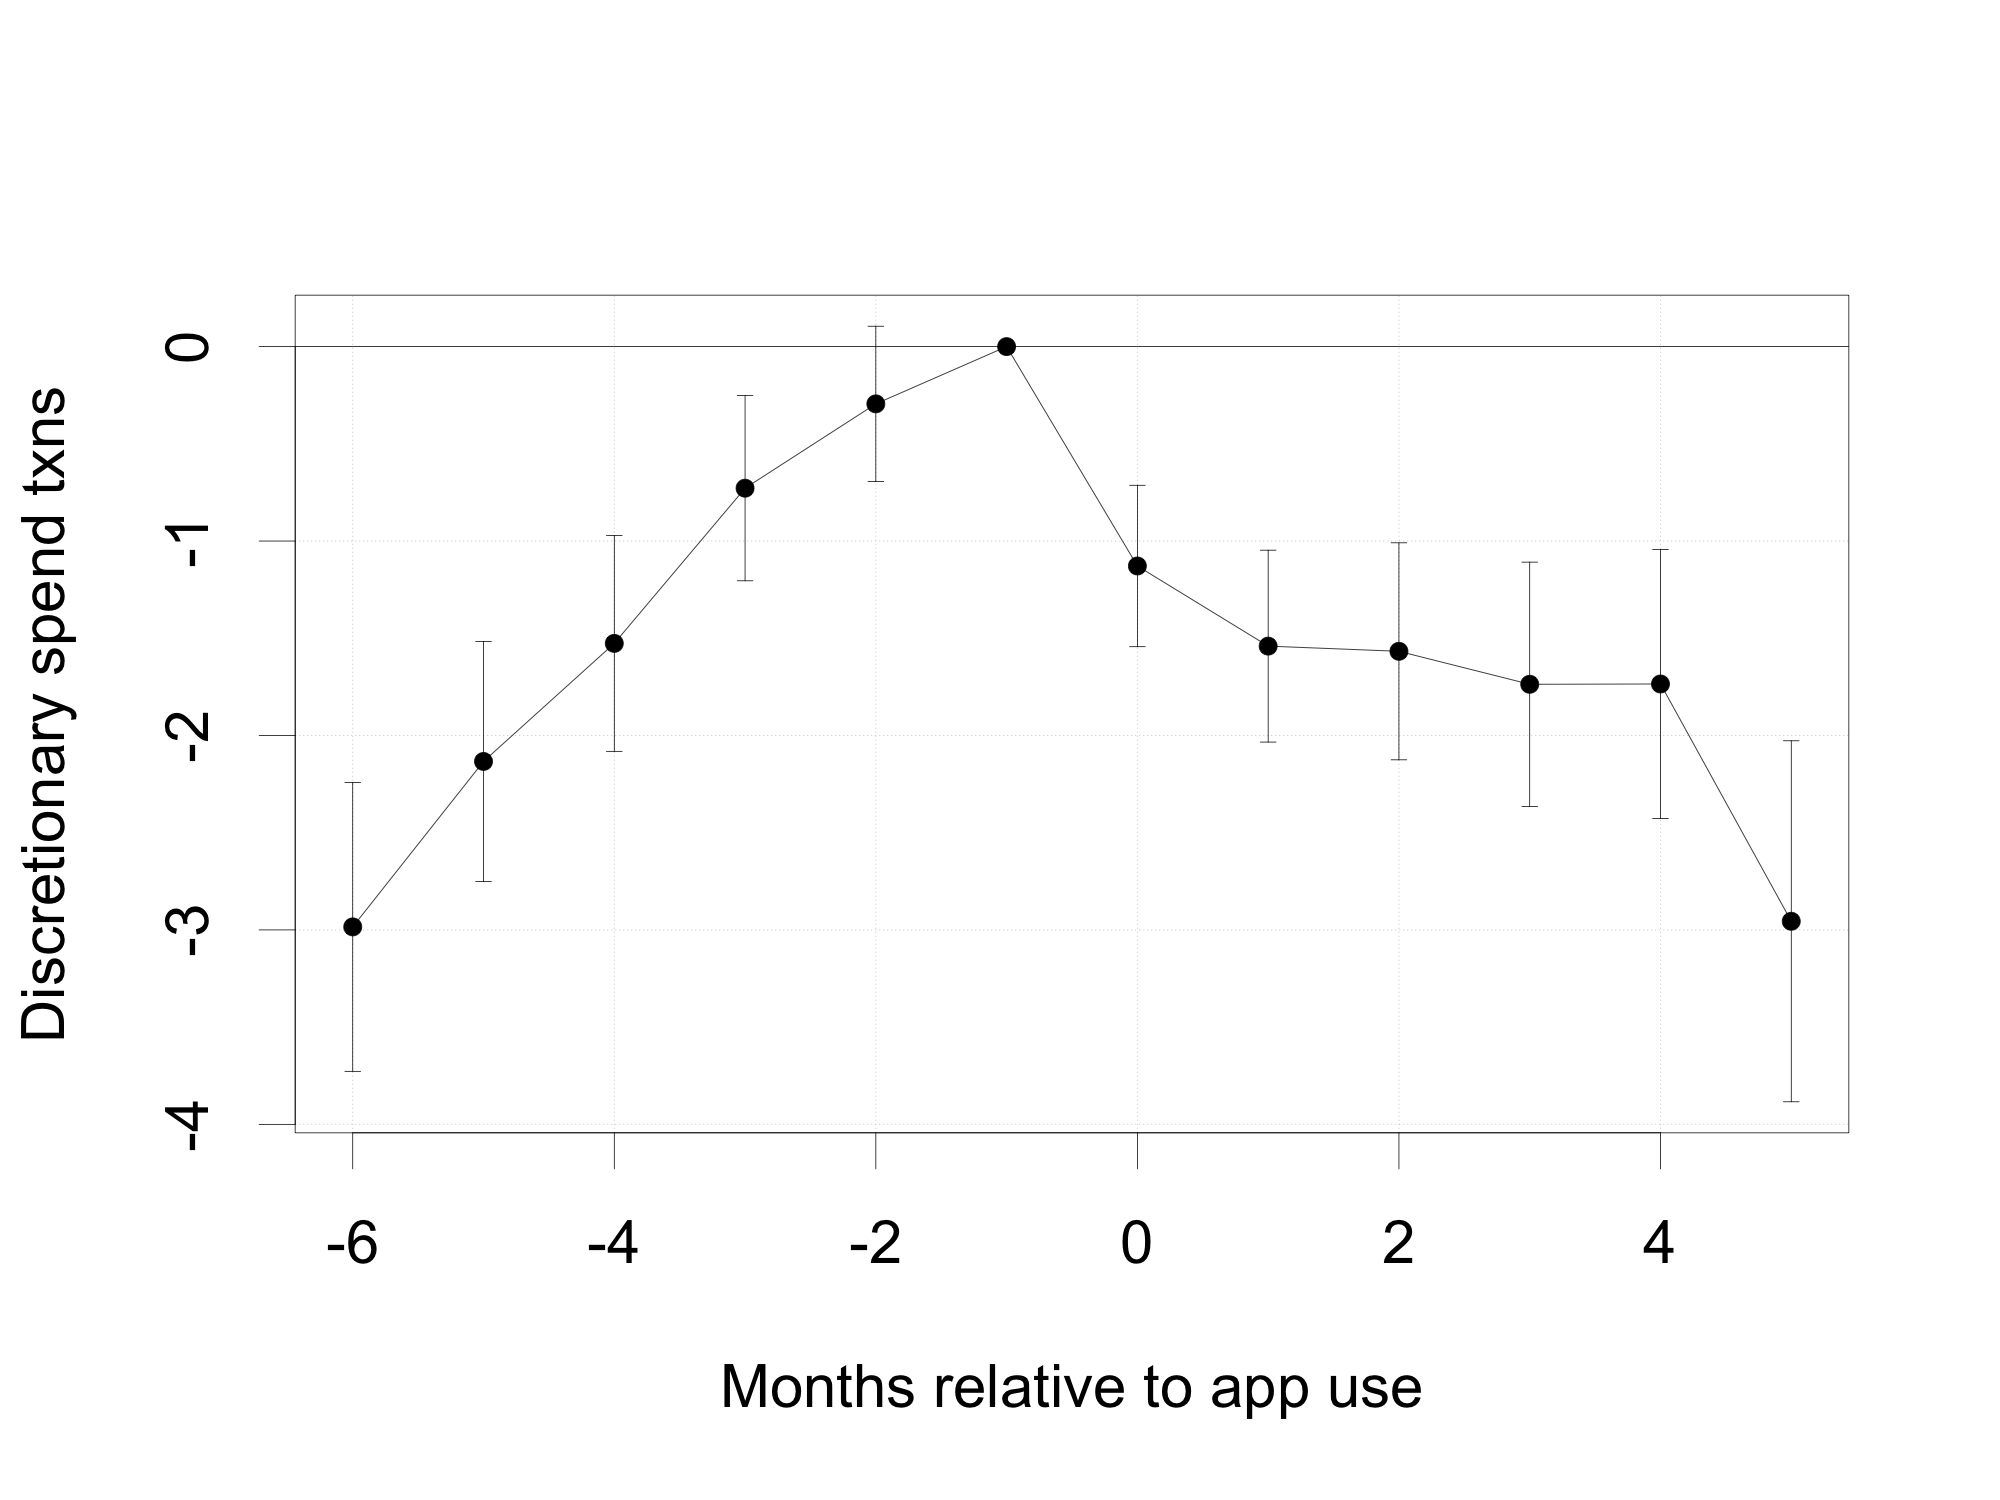
\includegraphics[width=.49\textwidth]{\figdir/dspend_count.png}
    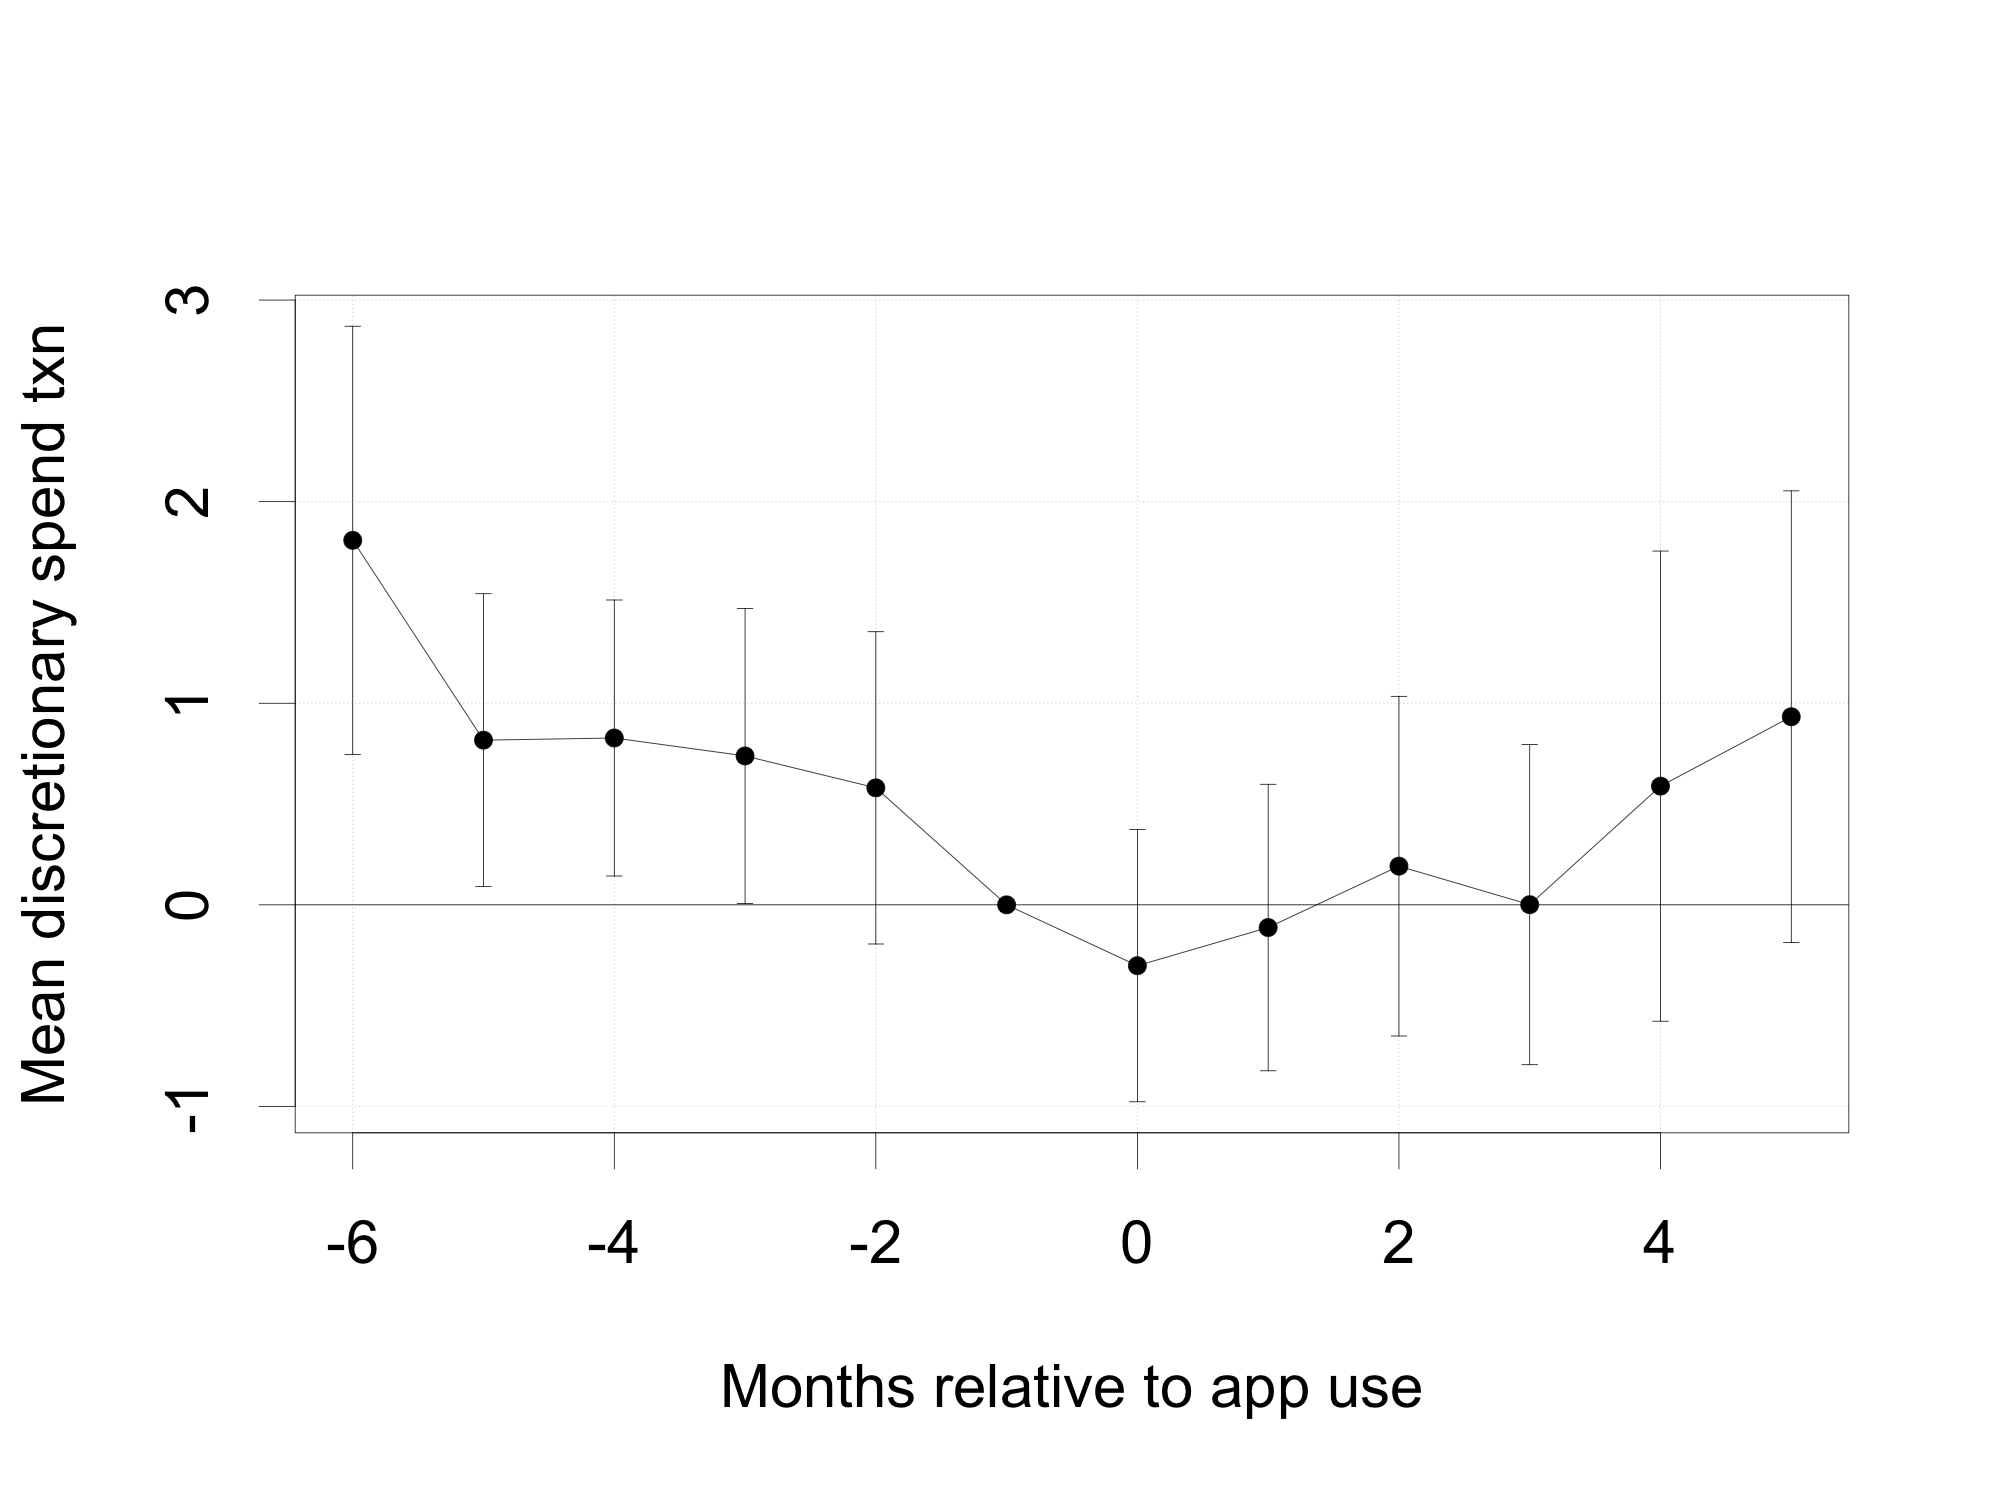
\includegraphics[width=.49\textwidth]{\figdir/dspend_mean.png}
    \fignote{\textwidth}{...}
\end{figure}

\begin{table}[htbp]
   \centering
   \tiny
   \begin{threeparttable}[b]
      \caption{\label{tab:intext} Intensive and extensive margins}
      \begin{tabular}{lcccc}
         \tabularnewline \midrule \midrule
         Dependent Variables:              & Has positive net-inflows & Positive net-inflows & Discretionary spend txns & Mean discretionary spend txn\\  
         Model:                            & (1)                      & (2)                  & (3)                      & (4)\\  
         \midrule
         \emph{Variables}\\
         Months relative to app use $=$ -6 & 0.02$^{***}$             & 68.33$^{**}$         & -2.98$^{***}$            & 1.81$^{***}$\\   
                                           & [0.01; 0.04]             & [0.10; 136.56]       & [-3.73; -2.24]           & [0.75; 2.87]\\   
         Months relative to app use $=$ -5 & 0.02$^{***}$             & 51.29                & -2.13$^{***}$            & 0.82$^{**}$\\   
                                           & [0.00; 0.03]             & [-26.47; 129.04]     & [-2.75; -1.52]           & [0.09; 1.54]\\   
         Months relative to app use $=$ -4 & 0.01                     & 1.77                 & -1.53$^{***}$            & 0.83$^{**}$\\   
                                           & [-0.01; 0.02]            & [-74.62; 78.15]      & [-2.08; -0.97]           & [0.14; 1.51]\\   
         Months relative to app use $=$ -3 & -0.01                    & -47.23               & -0.73$^{***}$            & 0.74$^{**}$\\   
                                           & [-0.02; 0.00]            & [-124.87; 30.40]     & [-1.20; -0.25]           & [0.01; 1.47]\\   
         Months relative to app use $=$ -2 & -0.01                    & -69.51$^{*}$         & -0.29                    & 0.58\\   
                                           & [-0.02; 0.00]            & [-141.13; 2.11]      & [-0.69; 0.10]            & [-0.19; 1.35]\\   
         Months relative to app use $=$ 0  & 0.00                     & 13.75                & -1.13$^{***}$            & -0.30\\   
                                           & [-0.01; 0.02]            & [-65.21; 92.72]      & [-1.54; -0.71]           & [-0.98; 0.37]\\   
         Months relative to app use $=$ 1  & 0.01                     & -21.45               & -1.54$^{***}$            & -0.11\\   
                                           & [-0.01; 0.02]            & [-96.59; 53.68]      & [-2.03; -1.05]           & [-0.82; 0.60]\\   
         Months relative to app use $=$ 2  & 0.01                     & -46.60               & -1.57$^{***}$            & 0.19\\   
                                           & [-0.00; 0.03]            & [-119.91; 26.70]     & [-2.13; -1.01]           & [-0.65; 1.03]\\   
         Months relative to app use $=$ 3  & 0.01$^{*}$               & -22.42               & -1.74$^{***}$            & 0.00\\   
                                           & [-0.00; 0.03]            & [-97.31; 52.48]      & [-2.37; -1.11]           & [-0.79; 0.79]\\   
         Months relative to app use $=$ 4  & 0.02$^{**}$              & -14.37               & -1.74$^{***}$            & 0.59\\   
                                           & [0.00; 0.03]             & [-89.61; 60.87]      & [-2.43; -1.04]           & [-0.58; 1.76]\\   
         Months relative to app use $=$ 5  & 0.02$^{**}$              & 28.69                & -2.96$^{***}$            & 0.93\\   
                                           & [0.00; 0.04]             & [-41.84; 99.21]      & [-3.88; -2.03]           & [-0.19; 2.05]\\   
         Month income                      & 0.00$^{***}$             & 0.06$^{***}$         & 0.00$^{***}$             & -0.00$^{***}$\\   
                                           & [0.00; 0.00]             & [0.04; 0.08]         & [0.00; 0.00]             & [-0.00; -0.00]\\   
         Month spend                       & -0.00$^{***}$            & 0.02$^{***}$         & 0.00$^{***}$             & 0.00$^{***}$\\   
                                           & [-0.00; -0.00]           & [0.01; 0.03]         & [0.00; 0.00]             & [0.00; 0.00]\\   
         Active accounts                   & 0.09$^{***}$             & 184.51$^{***}$       & 3.41$^{***}$             & -0.87$^{***}$\\   
                                           & [0.09; 0.10]             & [170.36; 198.66]     & [3.21; 3.62]             & [-1.21; -0.53]\\   
         \midrule
         \emph{Fixed-effects}\\
         User ID                           & Yes                      & Yes                  & Yes                      & Yes\\  
         Year-month                        & Yes                      & Yes                  & Yes                      & Yes\\  
         \midrule
         \emph{Fit statistics}\\
         Observations                      & 188,324                  & 188,324              & 188,324                  & 187,306\\  
         R$^2$                             & 0.28475                  & 0.11551              & 0.68049                  & 0.26390\\  
         Within R$^2$                      & 0.06323                  & 0.01277              & 0.17182                  & 0.01562\\  
         \midrule \midrule
         \multicolumn{5}{l}{\emph{Clustered (User ID) co-variance matrix, 95\% confidence intervals in brackets}}\\
         \multicolumn{5}{l}{\emph{Signif. Codes: ***: 0.01, **: 0.05, *: 0.1}}\\
      \end{tabular}
   \end{threeparttable}
\end{table}





\subsection{Subgroups}%
\label{sub:subgroups}
To analyse which groups benefit most from adopting Money Dashboard, we split
our sample by gender, generation, income quartiles, and pre-adoption savings
behaviour.

We define generations as follows: boomers were born between 1946 and 1964, Gen
X between 1965 and 1980, Millennials between 1981 and 1996, and Gen Z after
1997.\footnote{Based on age ranges provides by
    \href{https://www.beresfordresearch.com/age-range-by-generation/}{Beresford
Research}.}

Subgroup analysis: same Fig an Tab as in main analysis, but with line for each
subgroup. One figure for each of: gender, generations, income terciles,
per-adoption average savings tercile (inspired by \citet{carlin2017fintech},
see Fig 5 and Table 4).

See also section 6 in \citet{gargano2021goal}


